\documentclass[11pt]{article}
\usepackage{header}

\def\P{\mathbb{P}} % Probability
\def\d{\mathrm{d}}
\def\zt{\stackrel{\mathcal{Z}}{\leftrightarrow}}
\def\ft{\stackrel{\mathcal{F}}{\leftrightarrow}}
\def\Xhat{\hat{X}(z)}
\def\Yhat{\hat{Y}(z)}
\def\Xhatu{\hat{x}(z)}
\def\Yhatu{\hat{y}(z)}
\def\Hhat{\hat{H}(z)}
\def\zinv{z^{-1}}
\def\zn{z^{-n}}
\def\zpn{z^{n}}
\def\zl{z^{-\ell}}
\def\zpl{z^{\ell}}
\def\zN{z^{-N}}
\def\zpN{z^{N}}
\def\zopn{z_{0}^{n}}

\newcommand{\myparagraph}[1]{\paragraph{#1}\mbox{}\\}
\newcommand{\myparagrapht}[1]{\paragraph{#1}\mbox{}}
\newcommand{\submyparagraph}[1]{\subparagraph{#1}\mbox{}\\}
\newcommand{\submyparagrapht}[1]{\subparagraph{#1}\mbox{}}
\newcommand{\ze}[1]{z^{-#1}}
\newcommand{\Xshat}[1]{\hat{X}_{\text{#1}}(z)}
\newcommand{\Xphat}[1]{\hat{X}\left(#1\right)}
\newcommand{\Hphat}[1]{\hat{H}\left(#1\right)}
\newcommand{\pd}[2]{\frac{\partial{#1}}{\partial{#2}}}
\newcommand{\dv}[2]{\frac{\mathrm d{#1}}{\mathrm d{#2}}}
\newcommand{\pdv}[2]{\frac{\partial{#1}}{\partial{#2}}}
\let\originalmiddle=\middle
\DeclareMathOperator{\sgn}{sgn}

\setcounter{tocdepth}{5}
\setcounter{secnumdepth}{5}

\usepackage[table]{xcolor}
\setlength{\arrayrulewidth}{1mm}
\setlength{\tabcolsep}{18pt}
\renewcommand{\arraystretch}{2.5}
\newcolumntype{s}{>{\columncolor[HTML]{AAACED}} p{3cm}}
\arrayrulecolor[HTML]{DB5800}

\begin{document}
% \setcounter{section}{8}
    \title{CS 160 Lecture Notes}
    
    \thispagestyle{empty}

    \begin{center}
    {\LARGE \bf Lecture Notes}\\
    {\large CS 160 with Bjoern Hartmann}\\
    Spring 2023
    \end{center}
    
    \tableofcontents

    % Note that I use include over input to force new page!
    {\textbf{Acknowledgements}}
I would like to recognize and thank Professor Babak Ayazifar for all information contained in these notes. 

Thanks to Jonathan Pei and any others who helped me typeset this.

    \section{Tuesday, January 17th}
\subsection{Welcome to User Interface Design and Development}
It is a nice sunny day, you are relaxing on your vacation in Hawaii. Suddenly, you get an alert on your phone that a missile attack is incoming.

But then it is clarified that there was actually no threat and the message was sent in mistake.

How did this happen?

To answer that question, let us look at the UI: We have a dropdown menu with ambiguous acronyms and a confirmation that follows. However the confirmation that follows highlights the ``Yes'' option as if it is the default.

\subsection{Where did we start}
\subsubsection{The Commandline}
In the Command-line, we had a terminal. Now we have a desktop with icons! Modern UI is organized like a physical office: there's a file cabinet with files and a wastebasket.

\begin{important}
But we should not take the metaphor too far:

Making a 3D VR-ish desktop office on your computer has benefits and downfalls. One major downfall is: you are trying to represent 3D via a 2D screen.
\end{important}

\subsection{Course Staff and Communication}
Here is the CS 160 course staff for this semester!

Bjoern Hartmann: Instructor

Shm Almeda: TA

Peitong Duan: TA

Ace Chen: Reader

Hridhay Suresh: Reader

\subsection{Enrollment}
This class is oversubscribed with $\sim$100 seats total, split between CS 160 (undergrad) and CS 260A (graduate).

We usually see 5-10\% turnover, so if you're in the first 10 positions then you should keep up with the class. Otherwise the chance that you can take the class this semester is unlikely.

Luckily, you can take this class in the summer semester!

Alternatively:
\begin{itemize}
    \item DES INV 15: Design Methoology
    \item DES INV 25: UX Design (non-technical)
    \item IEOR 170: Human Factors
    \item INFO 213: UI Design and Development
    \item INFO 114/214: UX Research
\end{itemize}
are classes you can look into.

\begin{important}
This class has a heavy workload. If you are an EE/CS Major, you already know what upper-division CS classes are like. If you do not think you can handle it, you should drop ASAP to give others a fair chance to get in.

If you are beyond spot 10 on the waitlist, consider leaving now. Likewise if you do not have a seat/cannot see the screen.
\end{important}

\subsection{This Course}
is about reliably building very good interactive systems.

We focus on \textbf{interactions with and 
through intelligent systems.}

The goal of this class is to build a working \textbf{interactive 
prototype.} We do \textit{not} focus on scaling the class to millions of people, for that CS 169 will moreson help you with that -- CS 160 is more for the front-end.

We place emphasis on de-risking via \textbf{user testing} and working on rapidly prototyping.

\subsection{Human-Computer Interaction (HCI)}
Design, prototyping \& evaluation of UIs.

Human
\begin{itemize}
    \item End-user of program
    \item Others (friends, collaborators, coworkers)
\end{itemize}

Computer
\begin{itemize}
    \item The machine the program runs on
    \item Can be (and often is) split: clients \& servers
\end{itemize}

Interaction
\begin{itemize}
    \item User tells the computer what they want
    \item Computer communicates results
\end{itemize}

\subsection{User Interfaces (UI)}
What allows people to interact with computers \& the computer to communicate results.

Note that this can include hardware design (i.e. buttons).

\subsubsection{Why Study User Interfaces?}
\begin{itemize}
    \item In today's applications, an average of 48\% of the code is devoted to the user interface portion -- It's a major part of work for ``real'' programs (approx 50\%).
    \item You work on real software intended for others
    \item Bad UI costs money, lives (see Airplane crash into a canyon due to badly designed UI in autocomplete software that the pilot used), votes, etc
    \item UI is hard to get right -- people are unpredictable.
\end{itemize}

\subsection{Interface Design Cycle}
If you take away anything from this lecture, remember this:
\begin{center}
    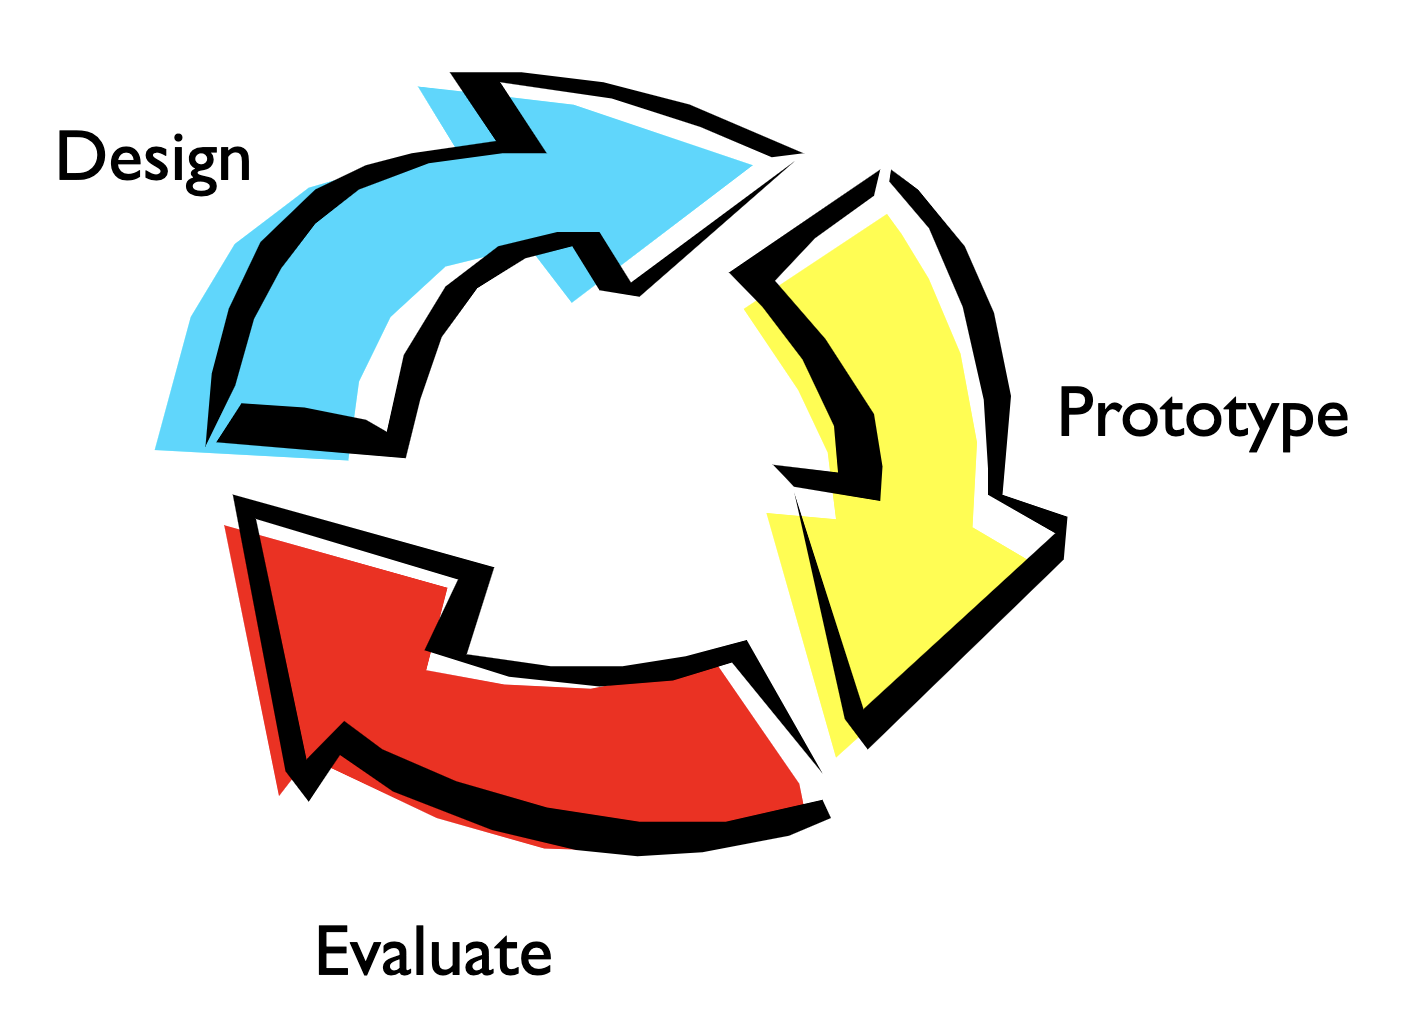
\includegraphics[scale=0.15]{lectures/wk1/img/cycle.png}
\end{center}

\subsection{Contextual Inquiry}
Observe existing practices.

Create scenarios of actual use.

Create models to gain insight  into work processes.

\subsection{Rapid Prototyping}
Low fidelity can be better as it is:
\begin{itemize}
    \item Fast, no attachment if you have to scrap it (if you were invested in it then you will stick with a bad UI due to the sunk-cost fallacy).
    \item No need to debug
\end{itemize}

\subsection{Evaluation}
\textbf{Test with real target users.}

Ask other CS 160 UI experts to check a UI for potential accessibility problems using the heuristics and conditions they learned to look for.


\subsection{Goals of the Course}
Learn to design, prototype, evaluate interfaces:
\begin{itemize}
    \item Discover tasks of prospective users
    \item Cognitive/perceptual constraints that effect design
    \item Techniques for evaluating an interface design
    \item Importance of iterative design for usability
    \item Technology used to prototype \& implement UI code
    \item Unique aspects of intelligent user interfaces
    \item How to work together on a team project
    \item Communicate your results to a group
\end{itemize}
These will likely be very important for future jobs.

$\hrulefill$

In other CS classes, you learn algorithms. Here we expect you to know algorithms and teach design.

\subsection{Teams}
\textbf{Instructors will form groups of 4-5 students (who are in the same section) in week 2 or 3.}

\subsection{Course Mechanics}
You must be comfortable with programming at the level of CS61B. 

Note: Individual programming assignments require you to write code in Javascript, HTML, CSS.

You must be able to attend class and one of the sections each week.

You must commit to working with your assigned team on your group project.

\subsection{Office Hours}
TBD

\subsection{Sections}
4 options: 
\begin{enumerate}
    \item 101 – Wed 11am-12pm, 540 Cory
    \item 102 - Fri 1-2pm, 310 Soda
    \item 103 – Th 10am-11am, 540 Cory
    \item 104 – Wed 2 -3pm, 320 Soda
\end{enumerate}
You MUST be able to attend one of the sections.

\textbf{Section starts next week}

1st half of the semester: Lecture material + Tech stack 
2nd half of the semester: Design critiques

\subsection{Readings}
Readings will be posted on bCourses.

Reading responses (recurring assignment)
You must post a substantial answer for each assigned reading, \textbf{by 10am before class} (so we can review them before class). 

Responses are the major factor in your \textit{class participation grade}.

\textbf{Your first reading response is due next Tuesday by 10am.}

\subsection{Grading}
\begin{enumerate}
    \item Participation – 10\% (Reading responses, class, Ed Discussions)
    \item Individual Assignments 20\%
    \item Two Midterms 30\%
    \item Group Project Assignments 40\%
\end{enumerate}
Note that we generally do the midterms in-class and this may not be accurate -- check bCourses.

\subsubsection{Late Assignments}
\begin{itemize}
    \item Most assignments will be due before class on the due date
    \item Individual assignments lose 20\% per day (weekend counts as one day)
    \item Group assignments will not be accepted late
\end{itemize}
 
    \section{Thursday, January 19th: The Design Cycle}
\subsection{UI Critique: Font Selection}
As a designer, one can always benefit from considering multiple interfaces and their respective benefits/tradeoffs.

When choosing what font you want text to be displayed in on Power point, you ahve 2 options:

\begin{enumerate}
    \item Have a flattened complete list of all combinations of font name, font family, and font weight, rendered in the system font.
    \item Have a dropdown that appears on hover with the family and weight, rendered in the font right there for you to see.
    \begin{itemize}
        \item This gives a visual inconsistency
        \item Most will not be used, so slows down the application, with minimal usage for non-graphic designers
        \item Does not show what numbers/symbols/etc other visual icons look like
    \end{itemize}
\end{enumerate}
This is not a world-ending decision but there are still tradeoffs. Arguably, neither got it right, which to use depends on the usecase and intended users.

\subsection{BCourses Logistics}
Make sure you are keeping up with the assignments listed there :D

\subsection{Where does design fit into the larger process?}
First, realize that there is both stuff before and after Design.

Before: R\&D -- they create the raw material, look into what matches user needs

After: Engineering (sometimes integrated with design, but sometimes separated), Sales -- marketing, feedback loop for re-design

\subsubsection{Oscillations over Project Lifespan}
The Design Cycle has a dual form which cycles over the number of ideas under consideration; however, this originally large number decays in magnitude to 1, as the project timeline progresses.

\subsubsection{Divergent vs Convergent Phases}
Divergent: Start with a lot of different ideas/prototypes

Convergent: Over time, you get more narrow and concrete on the concept of what you want to make.

\subsubsection{Waterfall Model (Software Engineering)}
A linear ``waterfall'' model where you can only go forward (and therefore don't allow anything to go backwards) does not work.

This model was used by the Federal Government (specifically wrt contractors) which is probably a key reason behind why their software sucks.

\begin{important}
This may not seem like that big of a deal, but as you get closer to shipping the project, these mistakes cost exponentially more to fix.
\end{important}

Iterative design de-risks your design cycle.

\subsubsection{Agile Software Development}
In Silicon Valley, you're more malleable to change. This differs from the similarly essenced iterative design in that this is more technical -- this is about writing code.

\subsection{Shopping Cart Video (from abc)}
In Palo Alto, CA, IDEO is a Design committee looked into making a new, better, shopping cart. \href{https://www.youtube.com/watch?v=M66ZU2PCIcM}{https://www.youtube.com/watch?v=M66ZU2PCIcM}

Student thoughts on how well they followed the design cycle in the video:
\begin{itemize}
    \item For the final evaluation video, it seemed kinda rushed.
    \item Evaluation happened earlier with post-it notes and multiple prototypes
\end{itemize}
Here Evaluation happened internal to the team (as opposed to user-tested).

They established themes through montages.

\subsection{Methods}
\subsubsection{Talking to people}
Talking to people is important, whether it be from asking stakeholders or interviewing experts.

\subsubsection{Stakeholder Map}
Being visual is important for designers, realize who is at risk as a consequence of your decision(s).

\subsection{Brainstorming}
\begin{enumerate}
    \item Sharpen the Focus
    \item Playful Rules
    \item Number your Ideas
    \item Build and Jump
    \item The Space Remembers
    \item Stretch Your Mental Muscles
    \item Get Physical
\end{enumerate}

\begin{shaded}
Aim for quantity, but hope for quality.
\end{shaded}

    \section{Tuesday, January 24th: Sketching}
\subsection{Logistics: Discussion Signup}
You can view your discussion assignment here: \href{https://tinyurl.com/cs160disc-sp23}{https://tinyurl.com/cs160disc-sp23}

\subsection{Sketching, Brainstorming, Critique}
\subsubsection{Case Study: Tesla Design}
Tesla Cards do stuff differently:
\begin{itemize}
    \item They have a large screen in the middle (in portrait mode -- vertically long)
    \item No longer physical buttons -- all touch screen
\end{itemize}

\subsection{Visions for the future of Car Designs}
\subsubsection{Apple Touchscreen Car Integration (from WWDC)}
All pixels all the time.

Benefits:
\begin{itemize}
    \item Shows more information
    \item Software will get updated
    \item You don't need to read a complex manual to use the car's basic features
    \item Cheaper than manufacturing buttons
\end{itemize}

\subsubsection{INEOS Grenadier}
All physical buttons.

Benefits:
\begin{itemize}
    \item More granularity in changing a knob by only a few degrees
    \item Does not require you to look at it to adjust
    \item Better in Mountain-like areas without WiFi
    \item Can be used with gloves/wet hands whereas a touchscreen cannot
\end{itemize}

\subsection{Sketching}
\subsubsection{Design Journals}
Can be a mixture of many different drawings/UI representations/etc.

See attached Drawing Pad for reference.

\subsubsection{Storyboard}
Disney uses this a lot:
\begin{itemize}
    \item Combines image frames with text to give a story without committing to all details
    \item Saves developer time
    \item Communicates a lot of information/content without being ``good'' drawings
\end{itemize}

\subsection{Brainstorming}
A particular technique for generating a lot of ideas (this is the divergent phase, not the convergent phase).

\begin{enumerate}
    \item Sharpen the Focus
    \begin{itemize}
        \item Make sure you have the right focus -- not too narrow or fuzzy.
        \item Widening your focus can allow you to consider innovative
    \end{itemize}
    
    \item Playful Rules
    \begin{itemize}
        \item Don't prematurely reject ideas because they sound too immature or playful
    \end{itemize}
    
    \item Number your Ideas
    \begin{itemize}
        \item This makes sure that no one person is attached to an idea
    \end{itemize}
    
    \item Build and Jump
    \begin{itemize}
        \item Exploration vs Exploitation
    \end{itemize}
    
    \item The Space Remembers
    \begin{itemize}
        \item Use a \textbf{lot} of space
        \item Giant Post-It Notes
        \item External Spatial Memory for your team (i.e. ``War Rooms'')
    \end{itemize}
    
    \item Stretch Your Mental Muscles
    \begin{itemize}
        \item Do puzzles
        \item Get immersed in the domain (go somewhere irl)
    \end{itemize}
    
    \item Get Physical
    \begin{itemize}
        \item Sketch
        \item Make Models
    \item Act out
    \end{itemize}
\end{enumerate}

\subsection{Critique}
\begin{important}
This is NOT for you to show off how great your project is -- you do not learn anything if you are just told that you did a great job.
\end{important}
It is also important not to insult (give feedback on the \textit{design}, not the \textit{designer} dispassionately), ask for specific alternates (instead of suggesting).

This differs from `Brainstorming' as `Critique' is more of an evaluation exercise, and less of a divergent mechanism.

    \section{Thursday, January 26th}
\subsection{Administrative Details}
Midterm Schedule set:
\begin{enumerate}
    \item Tue Feb 28
    \item Tue April 11
\end{enumerate}
\textbf{No Final Exam}

But Final Presentations will be on Wed or Thu during RRR week -- part of Jacobs Institute Design Showcase! (Schedule TBD)

\subsection{ChatGPT vs Google}
Similarity \& Differences between Web Search (Google) and chat-dialogue interaction (ChatGPT):
\begin{itemize}
    \item Search engines give multiple results which you can synthesize an answer from, whereas ChatGPT just gives an answer
    \item Google is helpful if you are in an explanatory phase
    \item Google gives more sources to cite from
    \item A singular answer from ChatGPT can be biased, whereas multiple sources from Google can allow us to diversify
    \item ChatGPT can be more detailed/step-by-step
    \item ChatGPT can answer questions that it hasn't seen before  in its corpus
    \item ChatGPT has memory, whereas search engines don't explicitly use previously queries
    \item Google has Images and other integrations, whereas ChatGPT is text-in text-out
    \item ChatGPT can be confidently incorrect
\end{itemize}

\begin{shaded}
`Go beyond intuition, observe target users in context to inform your design'
\end{shaded}

\subsection{XEROX PARC}
The first ``desktop'' computer came from here (IBM and Macintosh were influenced by it), though they were just a printer/copier company.

\subsubsection{XEROX 8200}
This was sold as a ``just click the button and you will be good to go'' but in reality, users found that it was too complicated.

Ever very smart people (ACM, Turing Award Winners, Chief Scientists at Powerset/Bing) were unable to operate the machine.

\subsubsection{Observation Techniques}
User Research:
\begin{itemize}
    \item Task Analysis
    \item Contextual Inquiry
    \item etc (Ethnography/Cultural Probes/Diary Studies)
\end{itemize}
Goal: Understand User's  Activities in Context

\subsection{Task Analysis}
\subsubsection{Case Study: BART Ticket Machine}
\begin{itemize}
    \item Lots of stickers, text, and numbers which overwhelms the user
    \item People read left-to-right so having earlier tasks more on the left in a noticeable position would be helpful
\end{itemize}

Solution:
\begin{itemize}
    \item Stratify into groups (i.e. tourists vs commuters)
    \item Age varies $\implies$ you cannot make the stand height too high or too low
    \item Make sure it is accessible to people in wheelchairs
\end{itemize}
\begin{important}
But this is wrong!
\end{important}
We should actually be talking to real users (found in BART stations) and ask them directly. You are a student so they will be more likely to talk to you than someone who is trying to sell you something; however, you should still make sure to properly compensate them for their time even if it is only a \$5 Starbucks Giftcard.

\subsubsection{Task Analysis Questions}
\begin{enumerate}
    \item Who is using the system?
    \item What tasks do they now perform?
    \item What tasks are desired?
    \item How are the tasks learned?
    \item Where are the tasks performed?
    \item What's the relationship between user \& data? 
    \item What other tools does the user have?
    \item How do users communicate with each other? 
    \item How often are the tasks performed? 
    \item What are the time constraints on the tasks? 
    \item What happens when things go wrong?
    \item etc
\end{enumerate}

\subsection{Old and New Tasks}
Now we have clipper cards, Paying with a phone, etc.

\subsection{Learning Tasks}
\begin{enumerate}
    \item What do they need to know?
    \item Do they need training?
    \item Experience, level of education and literacy
\end{enumerate}

\subsection{Where is the task}
...
Are their effects of other people (i.e. privacy concerns)
\subsubsection{Geography of the BART Station}
\begin{itemize}
    \item Loud
    \item Privacy
    \item Lighting is Dim
    \item Musicians and Rituals
\end{itemize}

\subsection{Other Tools}
Smartphones/laptops/Maps are artifacts whose integrations can be relevant for how users communicate.

\subsection{When things go wrong}
Make sure you have backup strategies

\subsubsection{Japanese QR Code Vending Machine}
This is a disaster as it required you to type out what product you want on clicking numbers multiple time + recieve an email 2FA (requires good internet):
\begin{important}
If your machine takes too long to work, then people will not use it. Sometimes people simply cannot use it.
\end{important}

Solution: Make sure tasks are specific.

    \section{Tuesday, January 31st: In-Class Team Brainstorm}
\subsection{Logistics: Assignments due!}
\begin{itemize}
    \item Team Brainstorm
    \begin{itemize}
        \item Aim for \~50 visual ideas!
    \end{itemize}
    \item Outside of class:
    \begin{itemize}
        \item Select initial course idea
        \item Target specific users (not students)
        \item Be creative -- you app should not be found in the app store!
    \end{itemize}
    \item Team Collaborative Plan
    \begin{itemize}
        \item Meet as a team
        \item Figure out team's strength/weaknesses
        \item Figure out how/when you'll meet
    \end{itemize}
    \item Individual Programming Assignment 1: Electric Time
    \begin{itemize}
        \item Simple web app
        \item Deploy, test, debug app locally
        \item Document \& showcase design + interactive features
        \item will be a Personal Transportation Conversion app
        \item Section (More HTML + JS) will help with starting this!
    \end{itemize}
    \item Thursday's Lecture: Conceptual Models + associated Reading Response
\end{itemize}

\subsection{Team Project}
\begin{shaded}
Be ambitious, yet realistic.
\end{shaded}
\subsubsection{Intelligent User Interfaces}
Example: Audio Fingerprinting a la Shazam.
\begin{itemize}
    \item Text-to-speech and Speech-to-text
    \item Translation
    \item Optical Character Recognition
    \item Image labeling, face, logo and landmark detection
    \item Image generation
    \item Classification and prediction using your own data
    \item Dialog systems (chatbots)
\end{itemize}
Example: Automatic Data Entry

Example: Automatic Text Translation

\subsubsection{Designing Inclusive Technologies}
\begin{shaded}
Abilities change over the course of our lives
\end{shaded}
Also recall that impairments can be:
\begin{itemize}
    \item Permanent (i.e. losing an arm)
    \item Temporary (i.e. arm injury)
    \item Situational (i.e. new parent with baby in one arm)
\end{itemize}

\subsection{In-Class Team Brainstorm: Meeting time!}
For the rest of the class please think of at least 50 app ideas that serve an underrepresented community.

The first group to finish will win free cookies!
\begin{shaded}
The winners were Group 8 consisting of Henry La, Karissa Wong, Priscila Figueroa, Rae Xin, and Rahul Shah.
\end{shaded}

    \section{Thursday, February 2nd: Contextual Inquiry, Conceptual Models 1}
\subsection{Case Study: Apple Watch}
You can have a modular home screen or one like traditional watches.

\subsubsection{Case Study: Calculators}
The 1990 HP-48SX calculator had an android emulator which mimicked it completely with overloaded buttons for easy familiarity at the cost of small hard to push buttons due to the touchscreen.

\subsection{Reminder: Assignments}
Tue Feb 7:
\begin{itemize}
\item Reading Response
\end{itemize}

Thu Feb 9:
\begin{itemize}
\item Team Collaborative Plan
\item Team Brainstorm
\end{itemize}

Mon Feb 13:
\begin{itemize}
\item Programming Assignment 1 – Electric Time
\end{itemize}

\subsection{Contextual Inquiry}
\subsubsection{Goals}
\begin{itemize}
    \item Go to where the customer works
    \item See what they do
    \item Talk to them about what they do
\end{itemize}
This gets you out of your perspective and see their tasks the way they do -- a mix between observing and interviewing.

\subsubsection{Context}
You want details not abstractions -- you want to be able to see their work live, in action.

When people are removed from their work environment they can only tell not show.

\myparagraph{Why not just interview folks?}
Folks may be used to inefficiencies and just accept things as ``that's just how things are done''

\subsubsection{Affordances}
The term affordance refers to the 
relationship between properties of a 
physical object and capabilities of a 
person, that determine how the object 
could be used.  

\subsubsection{Signifiers}
Signifiers help people figure out the 
affordances of objects without labels 
or instructions

\myparagraph{Case Study: Doors}
Q: How to make clear whether you push vs pull to open the door?

A: Make it so that there is only one clear way to do the intended action (i.e. no door handle implies push whereas

\subsubsection{Universal Signals}
Red means stop;\\
Green means go.

\subsubsection{Incorrect signifiers}
\begin{important}
Be careful: Signifiers may suggest affordances that do not exist.
\end{important}

    \section{Tuesday, February 7th}
\subsection{Conceptula Models (continued)}
We start at the \textbf{Design Model} and then go to the \textbf{System Image} which then iterates back and forth between itself and the \textbf{User's Model}.

It is important to realize that the User's Model is \textit{different} than the System Image -- the User cannot see your source code!

\subsubsection{Make Controls Visible}
Hidden side buttons or controls in hard-to-reach places will make it so that users don't know or won't use features.

\subsubsection{Don't overload the User}
``Too Much Visibility?'' is a thing and will make it had for the user to find the 1 button they want to press amongst the 200 available choices. Note that we will later formalize this with a function that measures visual search cost (More buttons $\implies$ longer processing time to find a button).

\subsubsection{Make Controls Clear}
A lot of seat controls have clear mappings from what you want to have happen to the action needed to make that a reality.

\subsubsection{Case Study: Stovetop Controls}
Which knob controls which burner on a stove is a classic UI question.

Contrary to common opinion, you do not actually need labels to make this unambiguously clear. All you need is to arrange the stoves in a non-linear manner and have the knobs be perturbed in the same manner:
\begin{figure}[H]
    \centering
    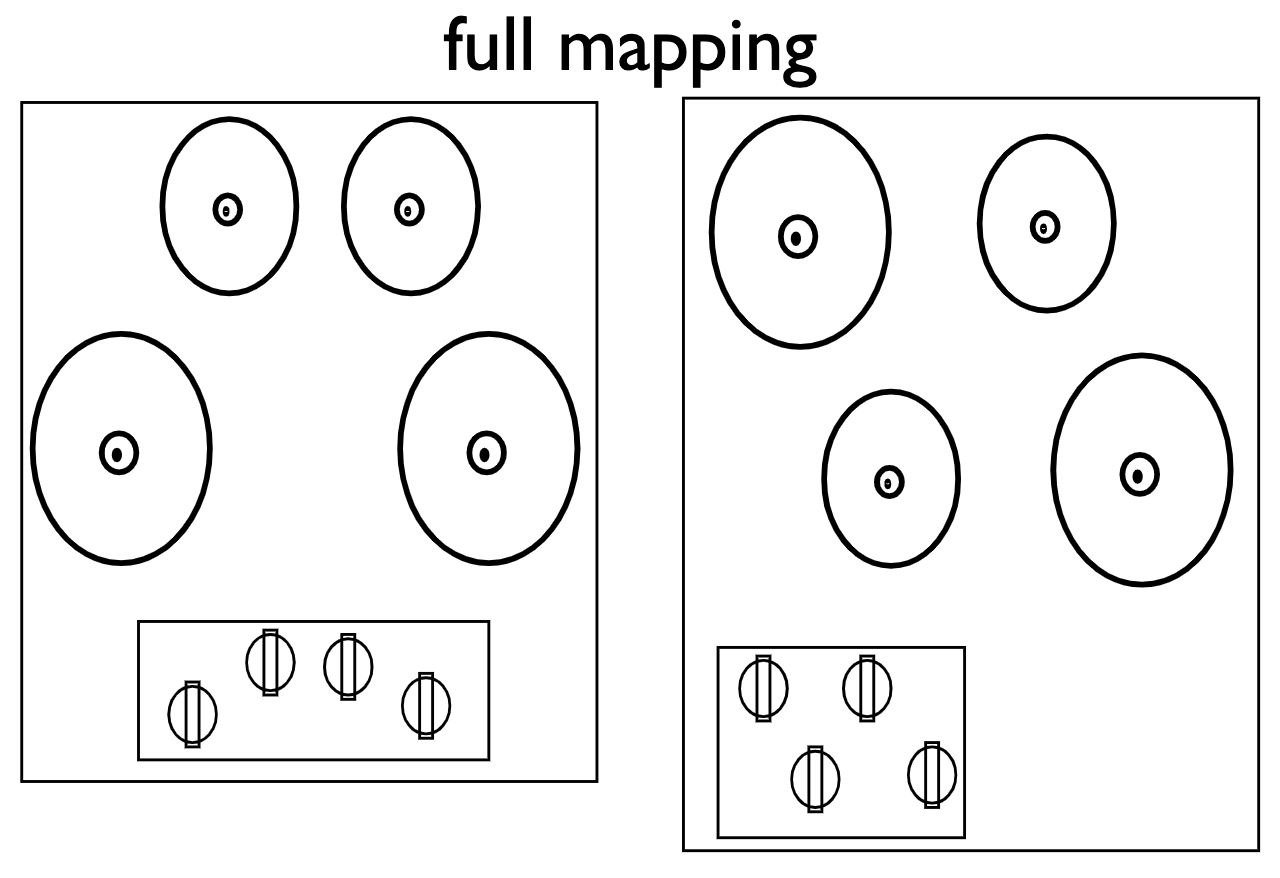
\includegraphics[scale=0.2]{lectures/wk4/img/stove.png}
    \caption{This is clear since the knobs are not packed in a horizontal line}
    \label{fig:stove}
\end{figure}

\subsubsection{Use Transfer Learning}
Knowledge from other domains can help users understand how new technologies can work. Laptops have keyboards in a layout that mimics those of typewriters to help people transition to newer technology.

\subsubsection{Provide Feedback}
\begin{shaded}
Q: Have you ever pressed a button more than once? If so, why?
\end{shaded}
The answer is likely that you did not recieve timely feedback that your input was registered (perhaps you did not press hard enough?).

Making sure you have low-latency is key for good UX.

\subsection{Action Cycle}
\begin{figure}[H]
    \centering
    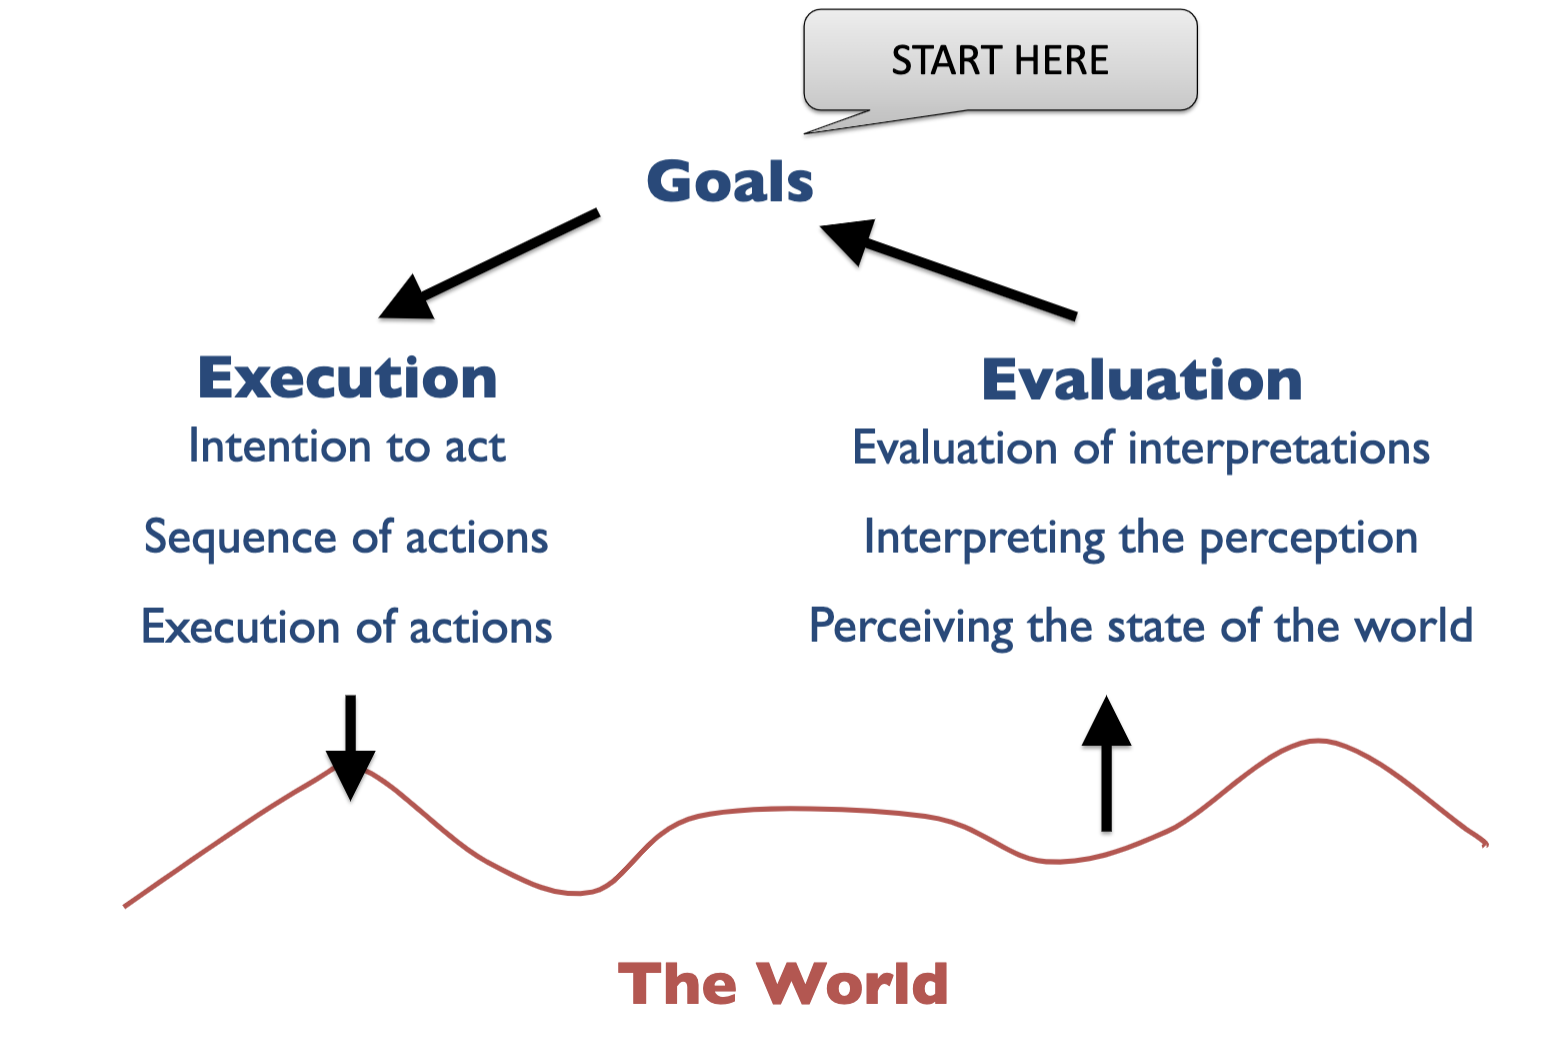
\includegraphics[scale=0.2]{lectures/wk4/img/action_cycle.png}
    \caption{This is a diagram of the Action Cycle}
    \label{fig:action_cycle}
\end{figure}

\subsubsection{Gulf of Evaluation}
Let us say that you are a Data Scientist who is trying to figure out some correlations.

If I can you some pairs of $(x, y)$ in an unsorted order this would be a very non-trivial task. Your first thought may be to re-order the data.

However what if I give you the data as a scatterplot. Then it may be a bit easier to immediately answer as we can use our perceptual systems.

\subsubsection{Gulf of Execution}
What if I ask you to draw some complicated shapes with a turtle drawing program?

This is non-trivial as you need to calculate some trigonometry. However if I gave you some `draw some shape' command then it would be much easier to execute this task. Note that the Execution is abstracted -- when coding we generally don't think about what is being put into each register in the generated Assembly code.

\begin{shaded}
    Gulf of Evaluation goes from  \textit{Mental Model} to the \textit{Real World}.
\end{shaded}

\subsection{Interface Languages}
\begin{shaded}
    An \textbf{interface language} is the set of actions a user can take in an 
interface. These actions have abstract \textit{meaning} and a concrete \textit{physical 
form}.  You can define its input language (provided by user to app) and 
its output language (provided by app to user)
\end{shaded}

\subsubsection{Semantic \& Articulatory Distance}
\begin{shaded}
\textbf{Semantic} distance reflects the relationship between the \textit{user’s 
intentions} and the \textit{meaning of expressions} in the interface languages.
% This is the distance between what you want 

\textbf{Articulatory} distance reflects the relationship between the \textit{physical 
form} of an expression in the interaction language and its \textit{meaning}.
% This is like what you have to do for 
\end{shaded}

\subsubsection{Case Study: Adding Autocomplete}
Q: If you added autocomplete to your app, would you be adding Semantic or Articulatory Distance? Would this narrow the gulf of execution or evaluation?

A: This is a trick question -- it can be both the gulf of execution (you need to type less keystrokes -- lower articulatory distance as you need to do less physical actions) or narrow the gulf of evaluation (as you get to see similar searches -- if you don't know how to spell something, your intentions can still be understood and met).

\subsubsection{Spell and Grammar Suggestions}
Gulf of evaluation (looking at what the UI shows you and interpreting ``did this meet my goal or not'') and semantic distances are both lowered since our intention gets matched up to the real world.

\subsection{Direct Manipulation}
An interface that behaves as though the interaction was with a real-world object rather than with an abstract system

Central ideas
\begin{enumerate}
    \item Visibility of the objects of interest
        \begin{itemize}
            \item If you open a phone, your apps are instantly viewable
        \end{itemize}
    \item Rapid, reversible, incremental actions
        \begin{itemize}
            \item You can undo actions
        \end{itemize}
    \item Manipulation by pointing and moving
        \begin{itemize}
            \item You can scroll between apps with ease
        \end{itemize}
    \item Immediate and continuous display of results
        \begin{itemize}
            \item There are no hidden states, or compiling, WYSIWYG (what you see is what you get)
        \end{itemize}
\end{enumerate}
GUIs were formed by HCI experts so that people in this room (i.e. non-CS majors) can work with technology.

\begin{important}
Note that if you have used something like \LaTeX\ then that is an example of something that is not direct manipulation.
\end{important}

Voice control (like Siri) narrows the Gulf of Execution.

\subsection{Metaphor}
\begin{shaded}
    \textbf{Metaphor} -- The transference of the relation between one set of objects to another set for the purpose of brief explanation
\end{shaded}

This can be useful to help clue users in what the functionality of an interface is and how it might be used.

Not all signifiers are metaphors -- metaphors are a type of signifier -- all metaphors lend themselves to affordances.

\subsection{Modes}
This can be useful in applications like Photoshop or Illustrator.

However this can be bad for the User as they need to remember what mode they are in. The SFO airplane crash we talked about in lecture 1 was due to the Pilot thinking they were on autopilot when they were not.

\subsubsection{Fixing the Problems with Modes}
\begin{itemize}
    \item Simply do not use modes
    \item Make it very explicitly clear which mode you are in
\end{itemize}

The easiest way to go about the second option is to make a redundant UI for the additional modes.

\subsubsection{Quasimodes}
You have to consciously and continuously take some action to stay in the mode.

The best example of this is the \texttt{Shift} key, where if you let go then you exit the mode. This makes sense as you more often than not want to type in lowercase.

This is different from the \texttt{Caps Lock} key which completely switches your mode (which can lead to the accident where you write a bunch of text in all caps, essentially unintentionally `yelling' at someone).

    \section{Thursday, February 9th: Human Information Processing}
\subsection{Galileo AI}
``Galileo AI creates delightful, editable UI designs from a simple text description. It empowers you to design faster than ever.''

\subsection{Review: Modes}
Last time we went over the Caps Lock key and how it was an example of a mode.

We also talked about quasimodes -- the discomfort of having to hold the Shift button down reminds you that you are still in the \textit{uppercase editing} mode.

\begin{important}
If you forget which mode you are in, you will have the source of numerous errors.
\end{important}

\subsubsection{Keyboard Modes: QWERTY, QWERTZ, AZERTY}
When typing in English vs German, the same buttons can map to letters and muscle memory can work against the User.

\subsubsection{Air France Flight 447}
In 2009, the plane switched modes due to a broken sensor, without alerting the Pilots. Then when the pilots tried to change the direction, they went into Gimbal Lock, from which they could not recover.

\subsection{Modeling Human Performance}
\subsubsection{Motivation}
This is useful to:
\begin{itemize}
    \item react to situations which we did not see -- broader applicability.
    \item A general solution by falling back on stuff we have seen before.
    \item Finally, we don't have to have observe things difficulty but we can extrapolate to unseen criteria
\end{itemize}
So you can react to designs \textit{without actually building them}.

\begin{important}
Note that even today we still don't have a perfectly comprehensive model -- we must still fallback upon the \textbf{design cycle}.
\end{important}

\subsubsection{Model Information Processor Theory}
This makes the assumption that humans take in data from a bunch of sensors (embedded systems) that go through a perceptual processor and the brain is just a distributed system consisting of multiple computers.
\begin{shaded}
Note that this is probably inaccurate but it predicts performance well.
\end{shaded}

\myparagraph{Perceptual Processor}
We take in features that are visual, audio, haptic, etc.

Our attention is selective and is very fast in dropping details. This is done via pre-attentive features (stuff that pop out at you) such as color (most prominently), shapes, curvature, size, convexity, and many more.
\begin{important}
Note that these cannot be combined -- pre-attentive features only work in isolation -- conjunctions do not work.
\end{important}

\begin{shaded}
Note that the perceptual processor has a cycle time for quantum experience of 100ms.

This is similar to what we see in CS61C w.r.t. how much can be processed, stuff faster cannot be processed.
\end{shaded}

\submyparagraph{Michotte Demonstration}
Causality falls off a cliff between 80 and 100 ms and after that, events are seen as indpendent.

\myparagraph{Memory}
Humans usually repack information as letters or numbers (abstract embeddings with meaning assigned to them) instead of series of pixels with brightness values.

\submyparagraph{Attention Span}
Humans can usually only remember at most $7\pm2$ things at once.

\begin{shaded}
    Attention Span: Interruptions > decay time.
\end{shaded}

The more things you are remembering, the longer the access time it will take to remember it will be.

This is analogous to how a CPU only has a limited number of registers for short-term memory.

\submyparagraph{Long-Term Memory}
In contrast to Short-Term attention span (STM), we also have a longer to access yet bigger Long-Term Memory (LTM).

\begin{shaded}
    There is no known limit for the capacity of Human's Long Term Memory.

    But it is hard to make sure the semantic encoding goes to LTM and not STM. Remembering/retrieving information is also an issue of concern.
\end{shaded}

\myparagraph{Cognitive Processor}
Humans are fundamentally not a multi-core machine -- you can only focus on one thing at a time -- you work in serial (multi-tasking is really just low-latency multiplexing).

\submyparagraph{Flight Eastern 401}
In 1972, the aircraft crashed due to the crew focusing on a `landing gear' indicator which overrode the `crash imminent' indicator to their senses, and made them miss the fact a crash ws imminent

\submyparagraph{Stroop Effect}
The meaning and visual infromation streams conflict and thus confuse your cognitive processor leading to higher latency.

\submyparagraph{Input Stratification}
You can calculate the net latency via adding each cognitive cycle for each processor (visual -- for reading, processing -- for classifying, motor -- for pushing a button, etc).

\begin{important}
    However this does not work since this is not accurate for complex tasks.
\end{important}

Different tasks have different difficulties. Use pre-attentive features or slow-motion to prolong videos if you want the User to see causality in something that occurs very fast.

\subsubsection{Stage Theory}
\myparagraph{Recognition over Recall}
Design for recognition %(given options) 
over recall (info reproduced from memory).

You have probably heard of Snow White \& the Seven Dwarfs but if you are asked to recall the names of the 7 Dwarfs it will probably be non-trivial to do so.

However if I give you a word bank and ask you to choose which are the names, then the task becomes much easier.

\subsection{Decision Making and Learning}
\subsubsection{Hick's Law: Decision Paralysis}
The time cost of taking a decision, $T$, depends on the number of options $n$:
\begin{equation}
    T = a + b\log_2(n+1)
\end{equation}
where $a, b$ are empirically derived constants. $a = \min$ time it takes to do the task (y-intercept), and $b$ = what human muscle group is being used and how quick that works.

This is why supermarkets make it hard to find products, as well as why they display so many products -- to overload your brain into thinking you need more than what you came for.

\subsubsection{Power Law of Practice}
Task time on the $n^{\text{th}}$ trial follows a power law:
\begin{equation}
    T_n = T_1 n^{-a} + c
\end{equation}
\begin{shaded}
    Main Idea: \textbf{You get faster the more times you do something.}
\end{shaded}
This means that it will take longer for visitors who are unfamiliar versus experts with the given technology. This also makes it hard to switch to new, unfamiliar, technologies as your muscle memory has already been built.

\subsection{Pointing}
\subsubsection{Fitts' Law: Distance and Target Size}
This is a foundational Model for any UI designer to know about.

\begin{equation}
    T = a + b\log_2(D/S+1)
\end{equation}
where $D$ = distance, and $S$ = size (and $[a, b] = $ [start/stop time, speed] are empirically derived constants).

\myparagraph{Index of Difficulty}
We can also formulate the Index of Difficulty:
\begin{equation}
    \text{ID} = \log_2(D/S + 1)
\end{equation}
This tells us that $T\uparrow$ as $D\uparrow$ \\
and that $T\downarrow$ as $S\uparrow$.

\begin{shaded}
    If we have a bigger button then it should be easier and faster to click on. This is a due to $S\uparrow$.
\end{shaded}

\myparagraph{Fitts' Law Tasks}
On a touchscreen, tapping and dragging are fundamental Fitts' Law Tasks.

On your laptop, Fitts' Law Tasks are moving your mouse pointer and clicking.

\subsubsection{The Power of Right-clicking: having options come to you}
Instead of having to drag your cursor across the screen, it is more optimal if you can have the list of options come to you. When you right click, a bar of options appears, this exploits Fitt's Law by making $D\to0$.


\subsection{Bandwidth of Human Muscle Groups}
\begin{center}
    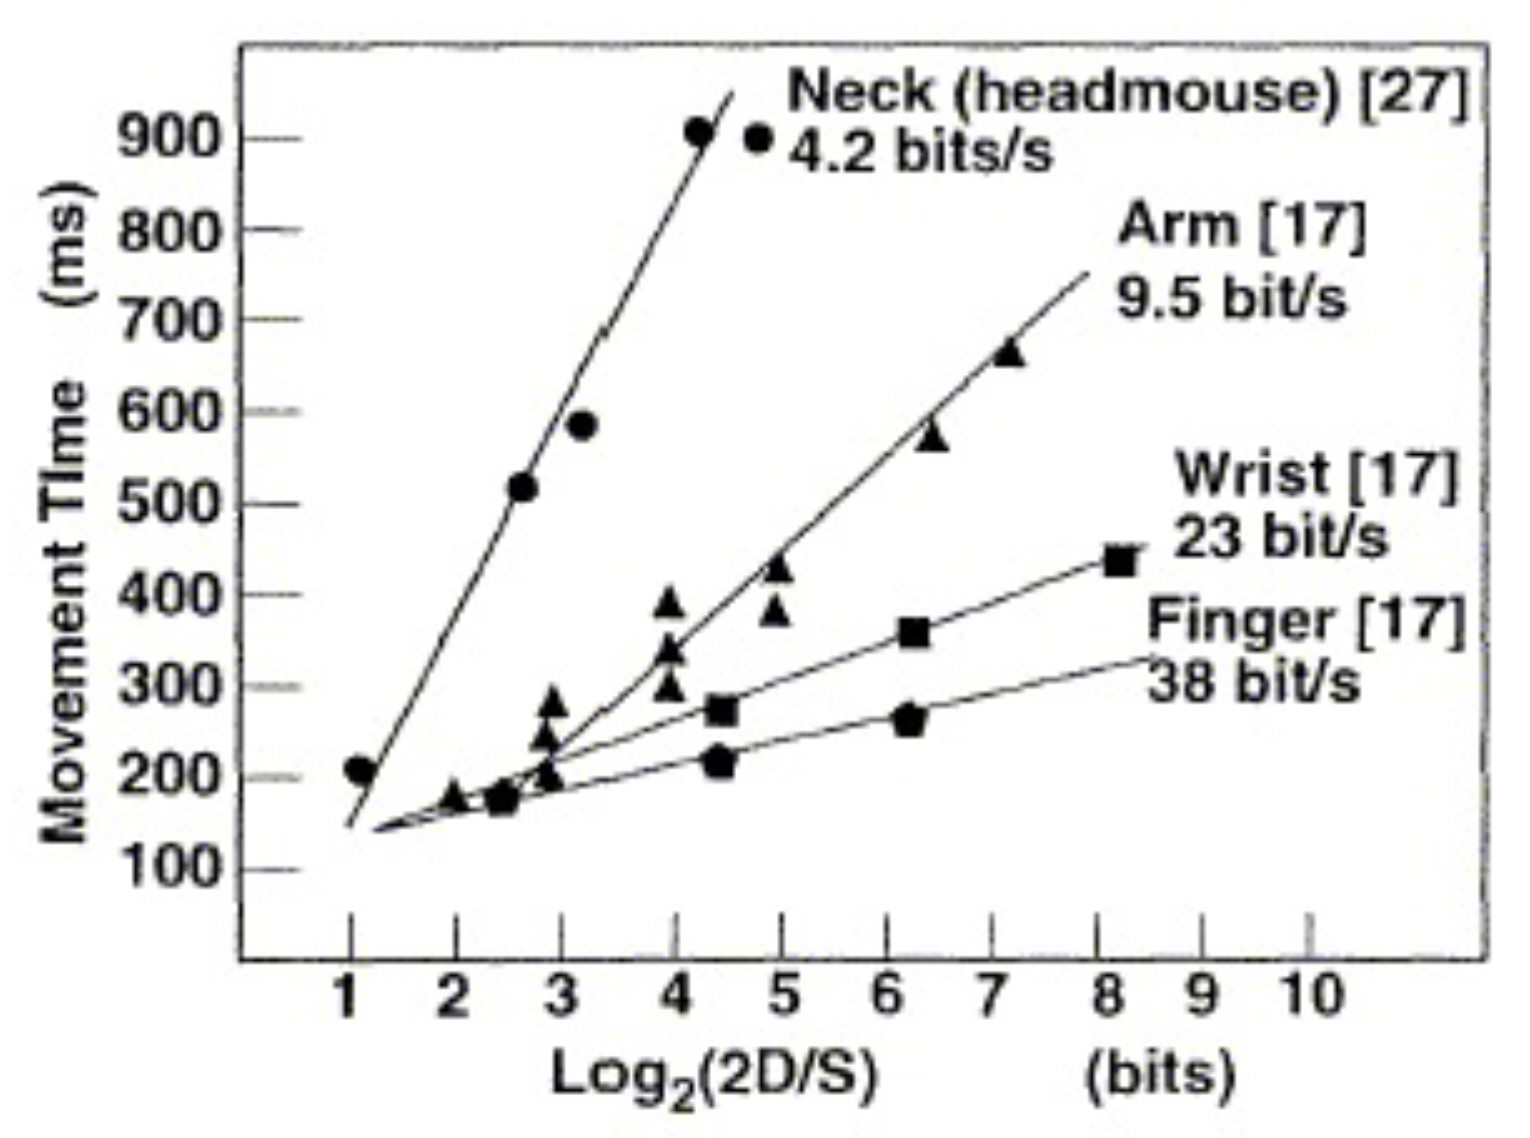
\includegraphics[scale=0.23]{lectures/wk4/img/bandwidth.png}
\end{center}
VR headsets are non-optimal as using fingers instead of neck to click on menus/swipe/move is a \>10x speedup.

    \section{Tuesday, February 14th}
\subsection{Interface Critique}
\subsubsection{Dual-Screen Devices}
Why should we have these?
\begin{itemize}
    \item More screen space
\end{itemize}

Why haven't we seen more of these?
\begin{itemize}
    \item Moving parts $\implies$ Mechanical Complexity $\implies$ Fall apart quicker
    \item More expensive $\implies$ lower return on investment
    \item Aesthetics: there will likely be a crease in the middle
    \item Not much marginal benefit for the additional pixels
\end{itemize}

\myparagraph{Microsoft Research: Codex}
This dual screen tablet computer worked well with embedded sensors to detect when the 2 phones were detached.

\myparagraph{Microsoft Research: Courier}
Courier was a prototype concept by Microsoft for a dual-touchscreen tablet. The device was conceived as being a digital notebook, consisting of two 7-inch touchscreens hinged together like a book, and running a custom operating system built primarily around handwriting input and a notebook-like journal for storing notes, images, and clippings from web pages.

\subsection{Administravia: Midterm 1}
You can take the exam any time in-between 9am Tuesday Feb. 28th to 8:59am Wed, online. You have 90min to complete the exam once it has started (unless you have accommodations).

This will be done via bcourses as a quiz with a mix of MCQ (where you can choose multiple options -- select all that apply) and short answer + open-ended questions (can range from a sentence to a paragraph or two). \\
This gives you an opportunity to show your understanding in a variety of ways.

\subsubsection{Scope}
Lectures 1 to 11 and associated readings.

Make sure to know basic HTML/JS/CSS concepts + terminology from assignments and sections.

\subsection{Input Devices}
\subsubsection{Text Entry: Keystroke Devices}
We have 2 criteria:
\begin{enumerate}
    \item Fast
    \item Low error rate (accurate)
\end{enumerate}

There are good since we can (generally) expect where keys will be on the keyboard,
\myparagraph{DVORAK vs QWERTY}
QWERTY was made to prevent typewriter jams, and was transferred to computers for transfer learning benefits.

DVORAK is not popular as people are used to QWERTY and learning new tech is hard (per the Power law of practice).

\myparagraph{Mobile Difficulty}
If buttons are too small, you run into the ``fat-finger problem''

Solutions:
\begin{shaded}
Multi-tap mappings: Press a key multiple times to get a letter

Candybar Phones implemented this (T9 had recognition for $43556\to$ `hello'):
\begin{center}
    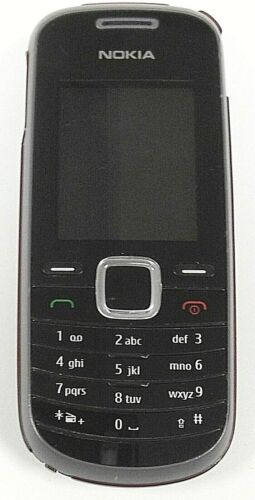
\includegraphics[scale=0.5]{lectures/wk5/img/candybar.jpg}
\end{center}
\end{shaded}

\myparagraph{Soft Keys}
Keys `f' and `j' have bumps on a computer keyboard but this tactile feedback information is lost on a touchscreen, which means you \textbf{have to} look at the screen to type.

\myparagraph{Drawing/Handwriting Recognition}
Why don't we use Drawing/Handwriting Recognition to input text?

Answer: it's slower than pressing keys

\myparagraph{Graffiti}
Custom alphabet with simplified symbols that are easier to recognize -- does not differentiate between lowercase and uppercase though.

\myparagraph{EdgeWrite}
Similar to Graffiti but Corner-based text input technique:
\begin{center}
    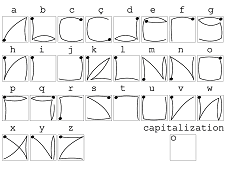
\includegraphics[scale=1]{lectures/wk5/img/edgewrite.png}
\end{center}

\myparagraph{Stroke writing}
You can also use backend algorithms to make this more accurate

\myparagraph{Speech Dictation}
This is $\sim$100 wpm. So why don't we always use this?
\begin{itemize}
    \item Privacy -- anyone nearby can hear
    \item Not socially acceptable -- to interrupt a quiet space with talking
    \item Can be hard to pickup \textit{only your} voice in a place with multiple people talking
    \item You have to know what you are going to say, ahead of time and that sort of `planning ahead' is more mentally demanding
    \begin{itemize}
        \item Editing previous words or even mistakes, is painful and adds more latency than doing the same operation on a keyboard.
    \end{itemize}
\end{itemize}

\subsection{Important Device Properties}
\subsubsection{Indirect vs Direct}
Direct: Input and Output space are unified (touchscreen)\\
Indirect: You're not pushing a button directly (mouse/trackpad/trackpoint)

\subsubsection{C:D Ratio}
For one unit of movement in physical space, how far does the 
cursor travel in display space?

Usually 1:1 for direct touch screen input.

\subsubsection{Device Acquisition Time}
Time between not using the device and starting to provide 
input

\subsection{Quadrature Encoding}
To use sensors for rotary encoding, you need $2$ bits of information:
\begin{enumerate}
    \item Which direction you are moving in
    \item How far you are moving in that direction
\end{enumerate}

\subsubsection{Optical Mice}
The physical mouse has hardware inside (a camera) which detects how much you have moved and which direction -- hundreds of times a second.

Fun fact: your mouse can be used as a (very bad) scanner.\\
It's not good as it doesn't have to be a repeatable proceeding device

\subsubsection{Trackpoint}
Lenovo Computers are known for having this red dot in the center.

\subsubsection{Resistive Touchscreens}
Cheap to manufacture  but only allows single-touch

\subsubsection{Capacitive Touchscreens}
Allow multi-touch

\begin{itemize}
    \item Direct input allows maximal screen space for mobile devices (ocular centrism).
    \item More degrees of freedom.
    \item ``Virtual input devices'' are adaptable.
    \item No extra pieces to lose or break (styli!)
\end{itemize}

\myparagraph{Exploit the edges}
Do not require users to explicitly click on some area/text. Instead allow the user to touch somewhere within some region an allow that to be sufficient to register an input click.

    \section{Thursday, February 16th: Input (contd.) and Prototyping}
\subsection{In the news: Adobe Acquisition of Figma}
Why did Adobe do this?
\begin{itemize}
    \item Although Adobe could and did have competing products that accomplished the same task, Figma had already accquired an active userbase
    \item To consolidate power: Adobe is \textit{the} company for 2-D Graphic Design
\end{itemize}

\subsection{Input Devices (contd.)}
\begin{important}
Why don’t interfaces designed for one input method work well for another?
\end{important}

Example: Android touchscreen apps on a Chromebook do not support multi-touch.

\subsubsection{Buxton's 3-State Model of Input}
\begin{tabular}{ |s|l| }
\hline
% \rowcolor{gray}
State & Description \\
\hline
0 & \textit{Out of Range:} The device is not in its physical tracking range. \\
\rowcolor{pink}
1 & \textit{Tracking:} Device Motion moves only the cursor. \\
2 & \textit{Dragging:} Device Motion moves objects on the screen. \\
\hline
\end{tabular}\\

One can consider applying Mouse/Touch Screen/Stylus on Tablet to the above.

\subsection{Prototyping Theory}
There multiple definitions of \textit{Prototype}:
\begin{shaded}
The means by which designers organically and evolutionarily learn, discover, generate, and refine designs. - Lim \& Stolterman.
\end{shaded}

Another definition is:
\begin{shaded}
A representation of a design, made before the final solution exist. - Moggridge, Designing Interactions.
\end{shaded}

The Industrial Design Process followed this with 8 steps.

This is an example of \textit{Observation and Contextual Inquiry}.

\subsection{The Value of Prototyping}
\subsubsection{Epistemic actions}
Experts rotate Tetris pieces more than novices as it is easier to visually see what the blocks look like when rotated than to mentallly rotate blocks.

\subsubsection{The Value of Surprise}
The Microwave Oven discovered ``by accident'' when a networking engineer at Raytheon noticed that the candy bar in his pocket would melt when he would get near to the magnetron radars that produced microwaves.

However the key point here is that the engineer \textit{took action}. They did not just wait for a surprise to come to them, they found something surprising and made a product out of it.

\subsection{Why Prototype?}
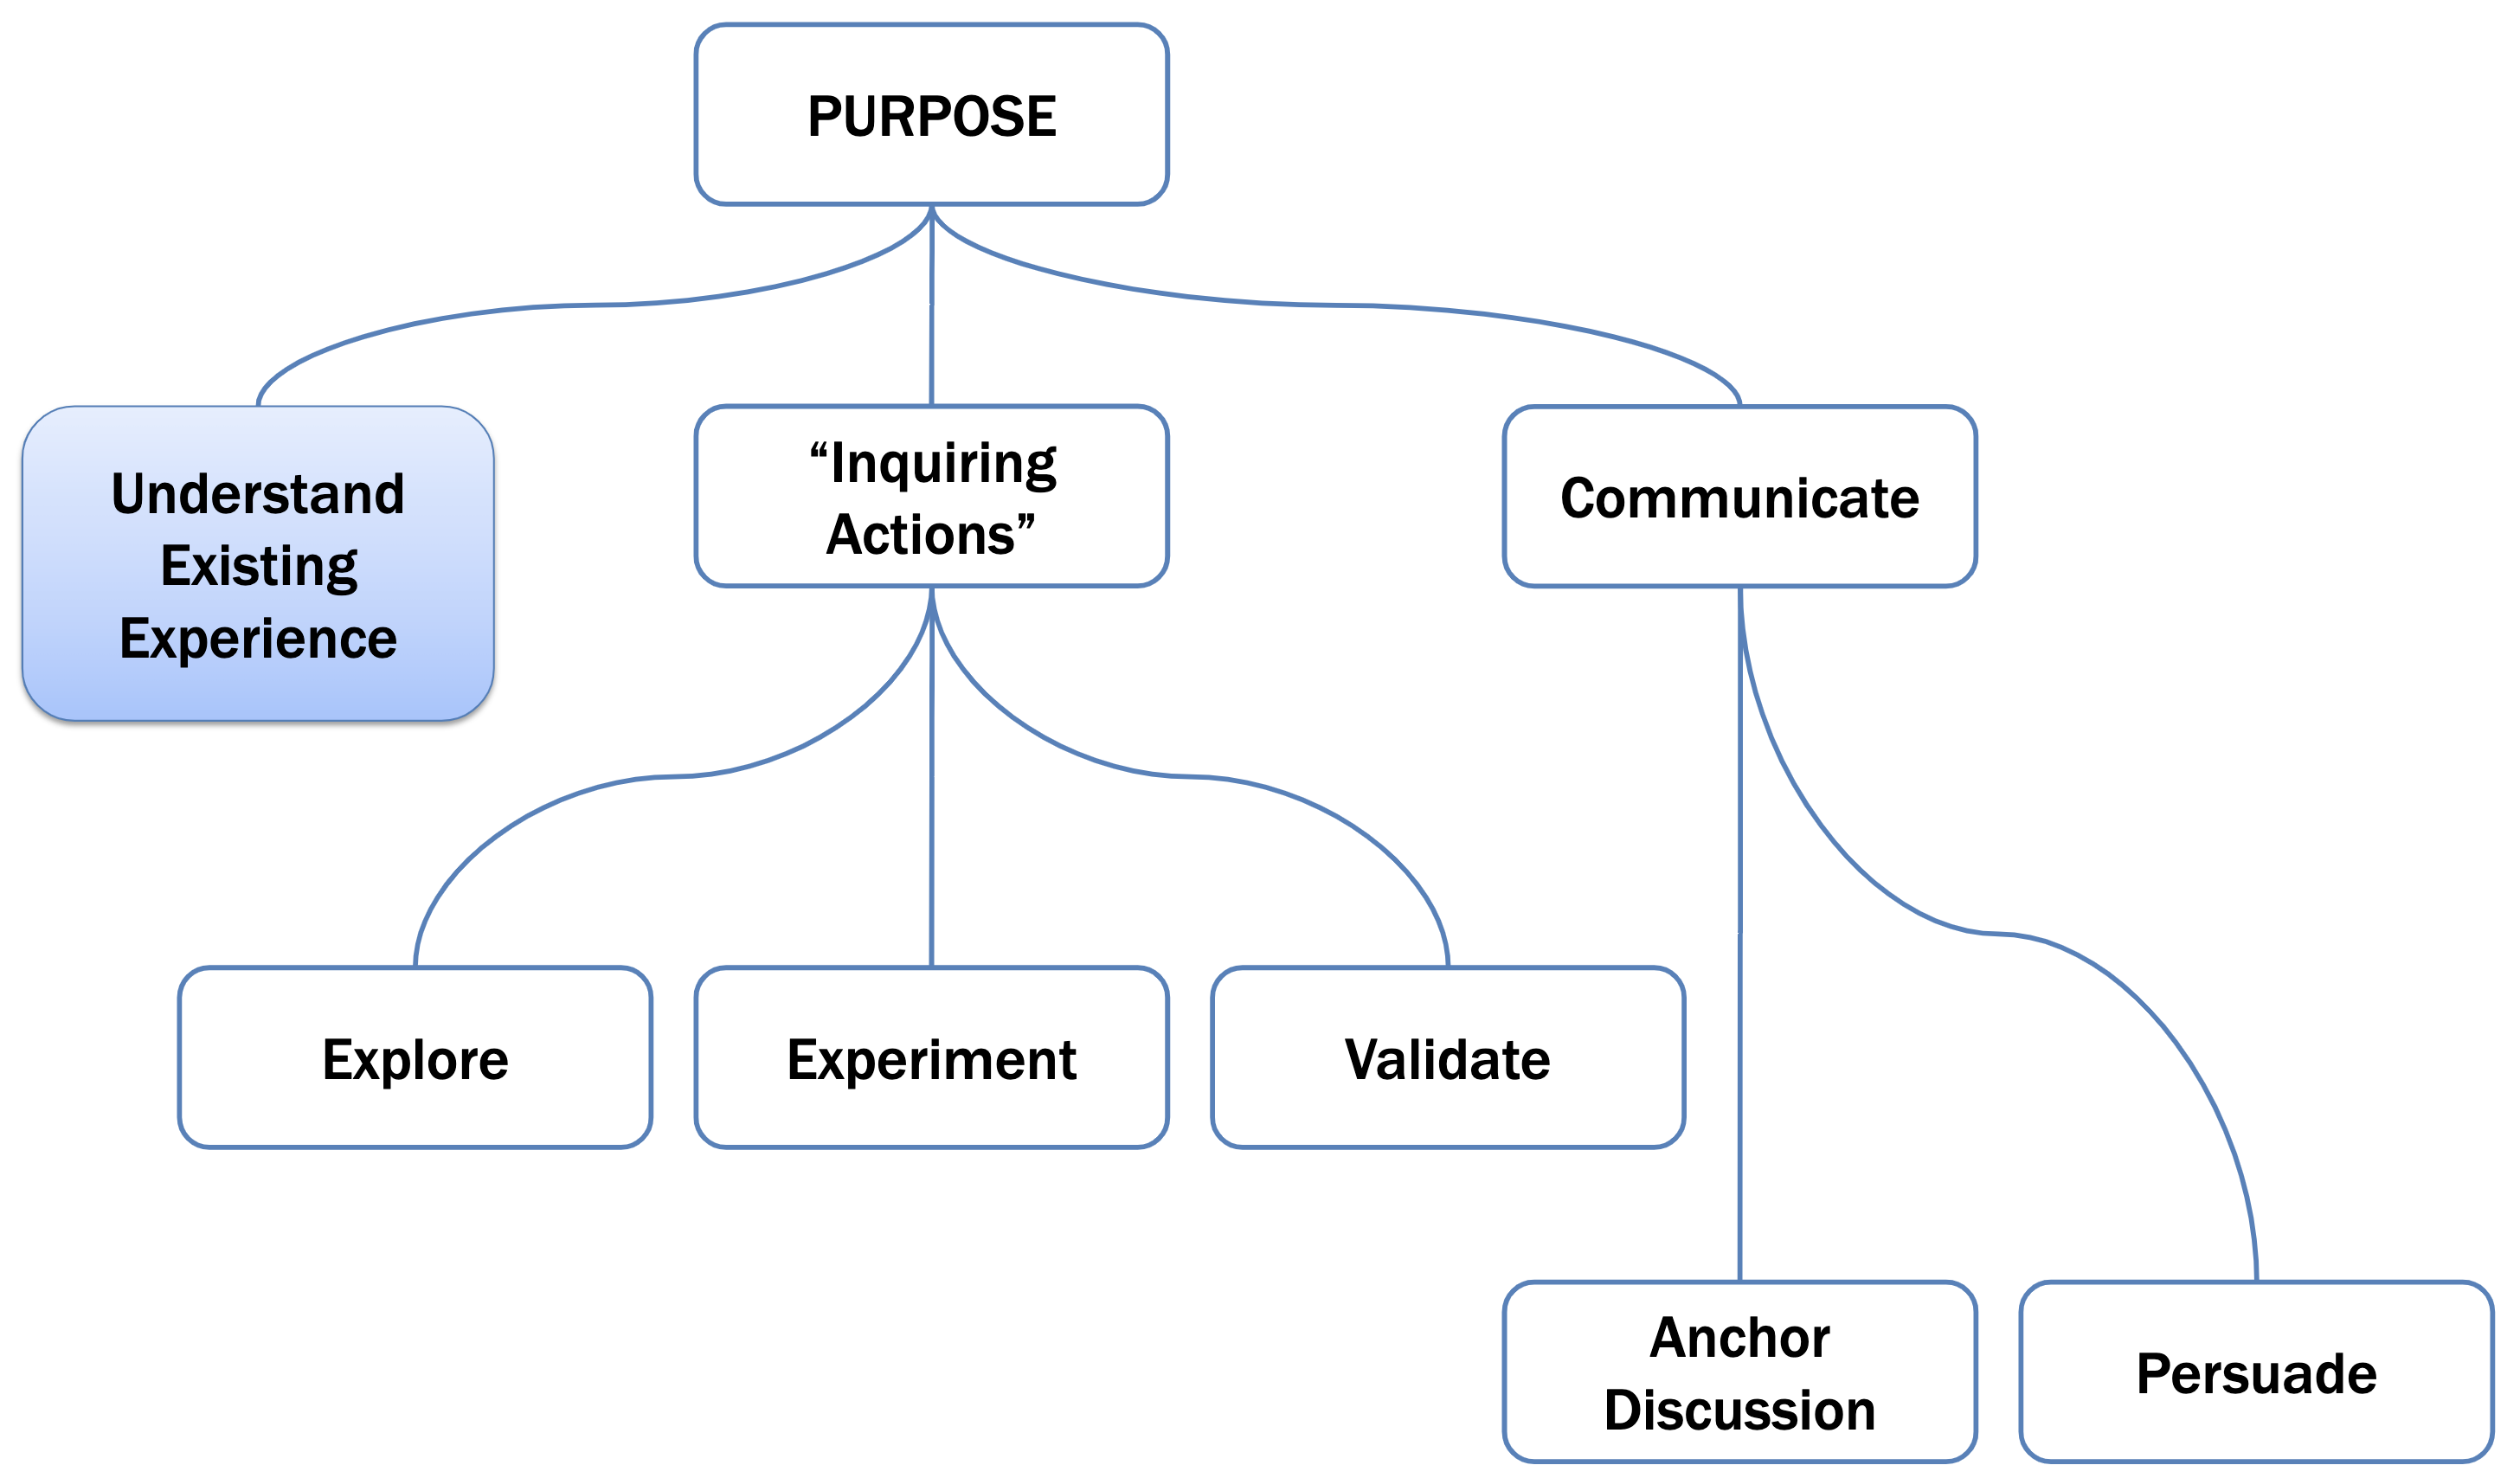
\includegraphics[scale=0.15]{lectures/wk5/img/why_prototype.png}\\
Microsoft had at least 5 different hardware prototypes of the Microsoft mouse, as well as hundreds of paper prototypes before a first version was officially released.

\subsection{Paper Prototyping}
It's hard to sink a lot of time into paper prototypes, so you won't get super attached to them (they are low fidelity).

Furthermore is is cheap and fast.

\subsubsection{Wizard of Oz Testing}
Have people test out your prototypes without letting them know what it is, allows you to get real feedback.

\subsection{Testing Device-Based Interfaces}
When conducting a test, it is preferable to have 3-4 testers.
\begin{itemize}
    \item \textbf{Greeter} - Puts users at ease \& gets data
    \item \textbf{Facilitator} - only team member who speaks
    \begin{itemize}
        \item Gives instructions \& encourages thoughts, opinions
    \end{itemize}
    \item \textbf{Computer} - knows application logic \& controls it
    \begin{itemize}
        \item Always simulates the response, w/o explanation
    \end{itemize}
    \item \textbf{Observer(s)} - Take notes \& recommendations
\end{itemize}
A typical session should be approximately \textbf{1 hour} as you have to:
\begin{itemize}
    \item Preparation
    \item The Test
    \item Debriefing
\end{itemize}

\begin{important}
    Make sure to record \textit{critical events}.

    Critical Events may also be moments when the user
    \begin{itemize}
        \item Got stuck
        \item Suddenly understood something
        \item Said ``That's cool''
        \item Said ``Ohhh'' etc. 
    \end{itemize}
\end{important}

\subsection{Prototyping in Software}
\subsubsection{Fidelity in Prototyping}
\begin{shaded}
    Fidelity refers to \textit{the level of detail}.
\end{shaded}

\begin{itemize}
    \item High fidelity: Prototypes look like the final product
    \item Low fidelity: Artists renditions with many details  missing
\end{itemize}

Paper Prototypes are low-fidelity. 

\myparagraph{Low-fidelity ``Informal'' design tools}
Examples:
\begin{itemize}
    \item DENIM (UC Berkeley)
    \item Balsamiq Wireframes
\end{itemize}
Goal is to be as rapid and flexible as physical tools.\\
Add benefits of digital media: Undo, copy+paste, resizing, etc.

\submyparagrapht{Advantages}
\begin{itemize}
    \item Takes only a few hours -- no expensive equipment needed.
    \item Can test multiple alternatives with the saved time -- faster iteration speed
    \item Can change the design as you test
    \item Especially useful for black-boxing hard to implement features such as Speech and handwriting recognition
\end{itemize}

\submyparagrapht{Disadvantages}
\begin{itemize}
    \item Can be hard to design at the proper scale / complexity  / information density of the real UI
    \item Need to re-create the interface in the target technology
    \item May not allow real-time end-user interaction
\end{itemize}

\myparagrapht{High-fidelity visual mockups}
\begin{itemize}
    \item Keynote, Powerpoint
    \item Flinto+Sketch
    \item Figma
    \item InVision
    \item Adobe Xd
\end{itemize}

\submyparagraph{Disadvantages}
\textbf{Distorts perceptions of the tester:}
\begin{itemize}
    \item Formal representation indicates “finished” nature
    \item People comment on color, fonts, and alignment
\end{itemize}

\textbf{Discourages major changes:}
\begin{itemize}
    \item Testers don’t want to change a “finished” design
    \item Sunk-cost reasoning: Designers don’t want to lose effort put into creating hi-fi design
\end{itemize}

\myparagraph{High-fidelity, fully-interactive prototypes}
Should look and behave like the final application.\\
Takes a lot of effort to build -- too little payoff -- only use as needed?

Example tools: 
\begin{itemize}
    \item HTML+CSS+Javascript
    \item Apache Cordova etc
\end{itemize}

\subsection{Video Prototyping}
Make sure to demonstrate each of the features/functionality your application will have.

Add structure to better explain content:
\begin{itemize}
    \item Begin with a title
    \item Follow with an “establishing shot”
    \item Create series of closeup \& mid-range shots, interspersed with title cards
    \item Place a final card with credits at the end
\end{itemize}

Can use stub-motion animation to help do this.

    \section{Tuesday, February 21st: Visual Design}
\subsection{Graphic Design}
\subsubsection{Communication}
\subsubsection{Interpretation}
\subsubsection{History}
Let's look at the start:\\
Materials are meant to be read and distributed, which means that you need to make sure texts are laid out in an understandable manner.

Terms such as upper case and lower case came from the separate cases used in printing presses -- \textit{terms which are still used today}.

\textbf{Main idea:} history influences the current state of design.

Churches or loyalties -- had lots of needs and wanted their words to be replicated. However after the 19th century, people have more disposable income so advertisements appear.

\subsubsection{Minimalism}
The London Underground is a great example of a simplistic yet `does its job' kind of logo which has withstood the test of time.

\subsubsection{Bauhaus Thinking}
Lots of Professors from the Bauhaus School of Art fled Nazi Germany and in going to the USA, etc they spread their thinking.

\myparagraph{Single axis of view}
A single vertical axis allows the user to read the text from top to bottom without confusion on where the next word(s) will be.

\myparagraph{Grid-based Design}
Every single element on the page is aligned to horizontal/vertical lines on an underlying grid.

Note that the grid does not have to be square or even axis-aligned, it just needs to be there to give structure.

\subsection{Visual Design}
\subsubsection{Corporate Identity}
IBM is a good example of a recognizable identity that is displayed on their posters as a brand mark.

\myparagraph{Logos}
This design of typefaces, size, color, etc is used even in Web Design -- think of the BBC news channel: their logo is recognizable and displayed on the top left of \href{https://www.bbc.com/}{https://www.bbc.com/}

\subsection{Product Design}
Product Design is about Form and Function.

\subsection{Streamlining}
This can be helpful but you should not take it too far.

\subsection{Form Follows Function}
\begin{shaded}
It is the pervading law of all things organic and inorganic,

Of all things physical and metaphysical,

Of all things human and all things super-human,

Of all true manifestations of the head,

Of the heart, of the soul,

That the life is recognizable in its expression,

\textbf{That form ever follows function.} This is the law.

- \textit{Louis Sullivan}
\end{shaded}

\subsection{Simplicity and Elegance}
\begin{shaded}
``Good artists borrow (from other artists), but great
artists steal!'' 

- \textit{Pablo Picasso}
\end{shaded}

\subsection{Simplicity}
Simple, minimalist, designs are often most effective. 

This is likely as there are less ways to interpret them (it has approachability, recognizability, and immediacy).

\subsection{Elegance}
The scrollbar is a good example of elegant design as it allows scrolling and indicates position in document.

\subsubsection{Reduction}
Only include essential elements.

\subsubsection{Regularization}
Use one set of shapes, colors, forms etc.

\subsubsection{Leverage}
Use elements in multiple roles.

\subsection{Unity}
One path to simplicity \& elegance is through unifying themes:\\
Forms, colors, components with like qualities.

Think of street signs.

\subsection{ Refinement}
Draw viewers’ attention to essential information.

Straighten subway lines to emphasize sequence of stops.

\begin{important}
Mistakes: Clutter \& Noise. Don't overdo it (especially with 3-D models on a 2-D screen).
\end{important}

\subsection{ Color}
\subsubsection{Color Spaces}
\myparagraph{Additive vs Subtractive}
Also known as RGB (red, green, blue) vs CMY (cyan, magenta, yellow).

These are used in Electronic Media and Printed Media respectively.

\subsubsection{Perceptual Organization}
There are 3-axes of color balance: Colorfulness, Hue, and Lightness. These parameterize our perception.

\subsubsection{Munsell Color Space}
Perceptually uniform book of painted chips

\begin{shaded}
Pro Tip:\\
Let Someone Else Pick For You
\end{shaded}

Some UI frameworks provide default themes... and color resources!

\subsection{ Gestalt Principles}
From Ware's 04 Paper:

\subsubsection{Figure/Ground}
Relative size.

\subsubsection{Proximity}
Introduce spacing/underlying grid.

Group related elements -- use size and typeface to allow scanning for groups.

\subsubsection{Similarity}
Can allow you to draw attention to one over the other $\in\{$rows, columns$\}$.

\subsubsection{Symmetry}
Bilateral symmetry gives strong sense of figure.

\subsubsection{Connectedness}
Connectedness overrules proximity, size, color shape.

\subsubsection{Continuity}
We prefer smooth not abrupt changes.

Connections are clearer with smooth contours.

\subsubsection{Closure}
\begin{center}
\begin{figure}[H]
    \centering
    
    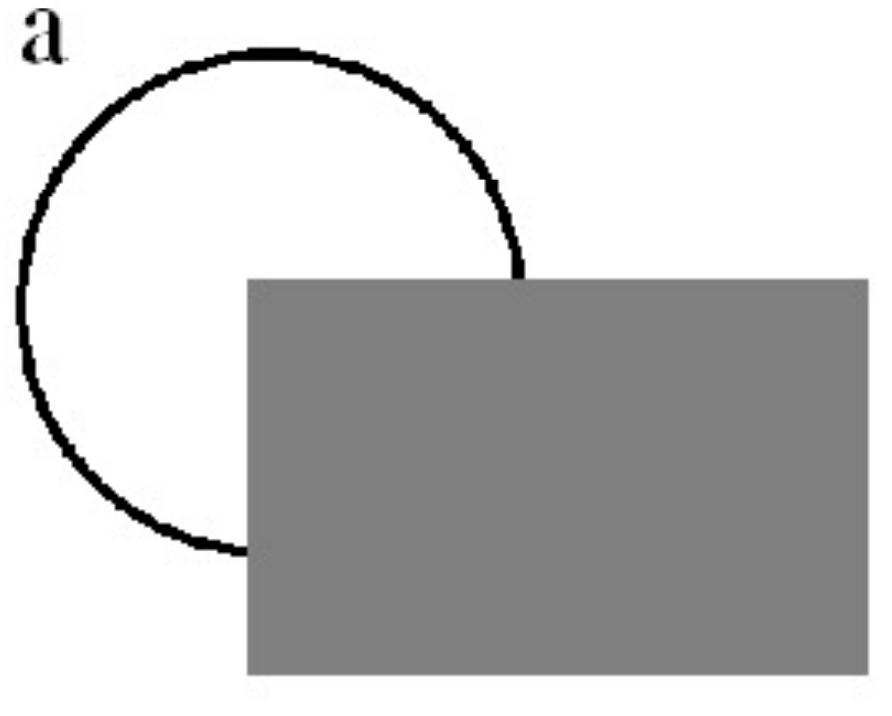
\includegraphics[scale=0.25]{lectures/wk6/img/a.png}
    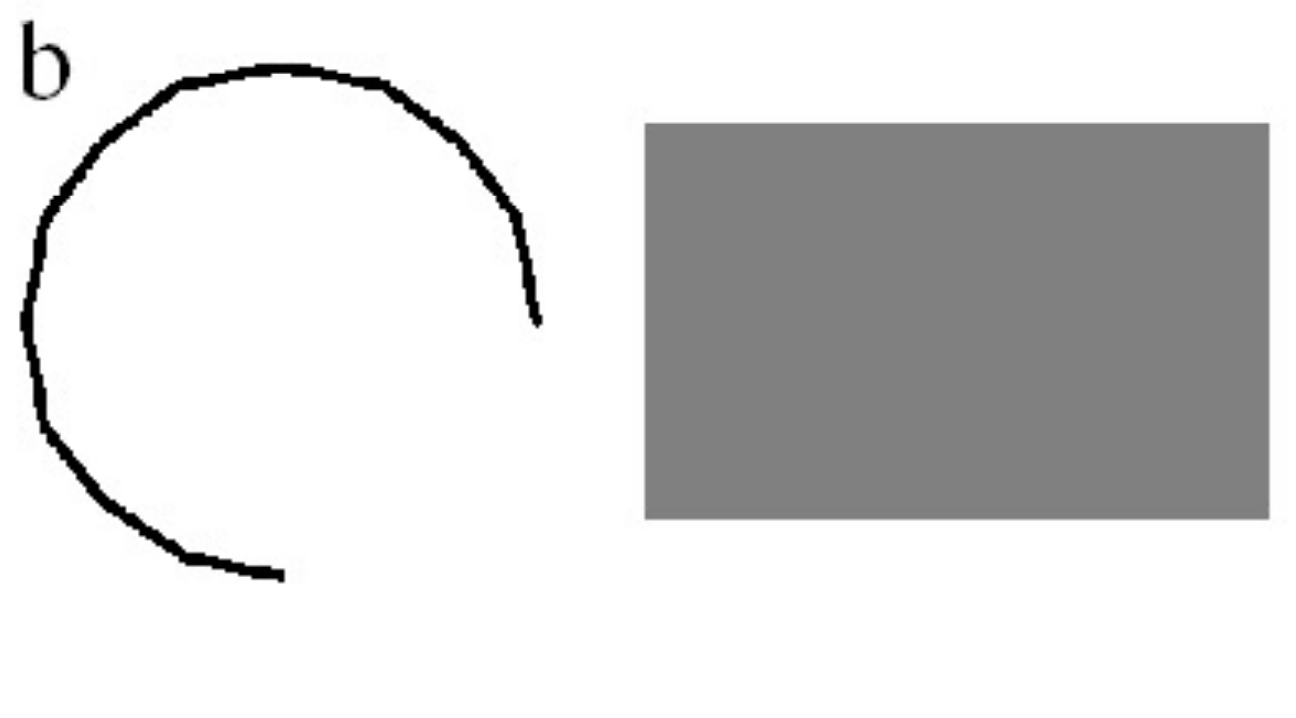
\includegraphics[scale=0.2]{lectures/wk6/img/b.png}
    
    \caption{We see a circle behind a rectangle, not a broken circle.}
\end{figure}
\end{center}

\subsubsection{Common Fate}
Dots moving together are grouped

\subsubsection{Transparency}

\subsection{ Fonts}
\subsubsection{Serif}
Flags/projections jetting off from the top of letters.

\subsubsection{Sans Serif}
Translates to ``Without Flags''

\subsubsection{Monospace}
A font where the space in between letters are fixed. The only use they have is for code/data/text where vertical alignment matters (i.e. Python code). 
\begin{important}
    You should not use this for long texts.
\end{important}
    % lec 12
\section{Thursday, February 23th: Midterm 1 Review}
\subsection{Logistics}
The quiz will be on bcourses under the ``Quizzes'' section. We will post a clarification form and have times on when we will monitor Ed posted.

\subsection{Composition}
Use grid systems -- what most web apps use!

Note that a text can be multiple grid cells but you mentally think of it wrt multiples of grid cells with whitespace in between.

\subsection{Alignment}
Every item on a screen has a relationship to the 
other items. Elements that are almost collinear 
should be aligned. 

Left, right and both-justified alignments create strong 
boundaries around a piece of text -- do not center allign text as you do not have an easy side border to read in a deterministic non-causal manner. 

Its best to stick with one kind of justification within 
a page.

\subsection{Common Mistakes}
\begin{important}
\begin{itemize}
    \item Arbitrary component positions and dimensions
    \item Random window sizes and layouts
    \item Unrelated icon sizes and imagery
    \item Poor alignment
\end{itemize}
\end{important}

\subsection{Summary}
What are the 3 stages of design cycle?

The Design Cycle is not everything.

As you go through the design cycle, you consider lots (>50 in brainstorming) but you end up shipping 1 product (divergent $\to$ convergent phases).

\subsection{Review}
\begin{shaded}
This has been added to the previous sections, as is relevant.
\end{shaded}

Good exam questions: 
\begin{itemize}
    \item If I tell you an object, tell me what its affordances are?

    \item Give an example of a mode that wasn't mentioned in lecture slides.

    \item Give an example of a task that follows a power law (i.e. typing).
\end{itemize}

    
    \section{Tuesday, February 28th: Midterm 1}
There is no class today due to the midterm!

\subsection{Next Class: Thursday, March 2nd}
\subsubsection{Work with your groupmates}
There is also no class today to give you an extra chance to work on your project!

    \section{Thursday, March 2nd}
\subsection{Work with your groupmates}
There is no class today!

    
    \section{Tuesday, February 28th}
\subsection{Information Visualization, Design Patterns}

EDA

Start with Color/Orientation/Shape so you're not that constrained for adding O/Q fetures in the future

Delta Stimulus

Loudness = approx 6.5

Heaviness and taste greater than 1 $\implies$ we overestimate those sensations.

Certain Visual Variables are better for comparisons.

    \section{Thursday, March 9th}
\begin{shaded}
Empirical studies are very expensive in terms of time and money
\end{shaded}
\subsection{Usability Testing}
    \subsubsection{Inspection Techniques}
    \begin{enumerate}
        \item Cognitive walkthroughs: put yourself in the shoes of the user. Check to see if the path users want to go is clear and logical. 
        
        \item Heuristic Evaluation: assess based on predetermined criteria / heuristics

        \item Other non-inspection techniques (mechanical turk)
    \end{enumerate}

    \subsubsection{Cognitive Walkthrough}
    \begin{enumerate}
        \item Get concrete goal
        \item get actions needed to complete said goal
        \item At each step as
        \begin{enumerate}
            \item Will the users know what to do?
            \item Will the user notice that the correct action is available?
            \item Will the user interpret the application feedback correctly?
        \end{enumerate}
    \end{enumerate}

    \subsection{Example: Find a book in a library}

    \begin{enumerate}
        \item find the library website
        \item find location of said book
        \item complete search form
        \item parse through to find latest edition
        \item click to get to the book's page
        \item find library and call number
    \end{enumerate}

    \subsubsection{Heuristic Evaluation}
    \begin{enumerate}
        \item Heuristic: rules of thumb that describe features of usable systems
        \item Example: Minimize user's memory load
        \begin{enumerate}
            \item get small number (3-5) people together to look at the UI separately
            \item give them list of heuristics
            \item get them to evaluate your design 
            \item aggregate findings of the independent evaluators and discuss
        \end{enumerate}
        \begin{enumerate}
            \item H2-1:Visibility of system status 
            \item H2-2: Match system and real world
            \item H2-3: User control and freedom
            \item H2-4: Consistency and standards
            \item H2-5: Error prevention
            \item H2-6: Recognition rather than recall
            \item H2-7: Flexibility and efficiency of use
            \item H2-8: Aesthetic and minimalist design
            \item H2-9: Help users recognize, diagnose, recover from errors
            \item H2-10: Help and documentation
        \end{enumerate}
    \end{enumerate}

\paragraph{Visibility of system status}
\begin{enumerate}
    \item Spiny ball
    \item buffering circle
    \item provide redundant information for each decision a user makes (do you want to save changes $\implies$ your changes will not be saved if you don't)
\end{enumerate}

\paragraph{Match System and World}
\begin{enumerate}    
\item follow real world conventions
\item pay attention to metaphors
\item Ex: used to drag floppy disk to trash to eject it. Did not line up with what trash usually does (data deletion)
\end{enumerate}

\paragraph{User control and freedom}
\begin{enumerate}
    \item users don't like being trapped
    \item give them freedom to choose to cancel, escape, universal undo (ctrl-z), postpone, etc.
 
\end{enumerate}

\paragraph{Consistency and standards}
\begin{enumerate}
    \item don't violate standards since they will behave according to how they expect things to behave
    \item example: put a word in a rounded rectangle implies its a button. People will click it.
\end{enumerate}

\paragraph{Error prevention}
\begin{enumerate}
    \item Check for errors (are you sure you want to do that)
    \item visual metaphors can help clear up incongruities
    \item types of errors: slips (right plan, bad execution) and mistakes (wrong plan, good execution). 
\end{enumerate}

\paragraph{Recognition over Recall}
\begin{enumerate}
    \item People are good at recognition and bad at recall
    \item Example: open recent files tab 
\end{enumerate}

\paragraph{Flexibility and efficiency of use}
\begin{enumerate}
    \item Experts want to save time
    \item Example: keyboard shortcuts, autocomplete 
\end{enumerate}

\paragraph{Aesthetic and Minimalist Design}
\begin{enumerate}
    \item Don't overload screen with information. Give them "details on demand"
    \item Occam's razor: remove or hide irrelevant or rarely needed info
    \item Present information in natural reading order (read left to right, top to bottom
\end{enumerate}

\paragraph{Help users diagnose recognise }
\begin{enumerate}
    \item When errors happen, help the users answer the "what do I do next?" question
    \item write good error messages that are descriptive and offer solutions
    \item Let them undo at every step  
\end{enumerate}

\paragraph{Provide help and documentation}
\begin{enumerate}
    \item easy to search
    \item focused on tasks
    \item list concrete steps to carry out
    \item not too long
    \item examples \begin{enumerate}
        \item tutorials
        \item reference manuals
        \item tool-tips
        \item "whats this" cursor
        \item search help bar
    \end{enumerate}
\end{enumerate}

\subsection{Heuristic Evaluation Steps}
\begin{enumerate}
    \item Pre-evaluation training
Provide the evaluator with domain knowledge if needed
2) Evaluation
Individuals evaluate interface then aggregate results
Compare interface elements with heuristics
Work in 2 passes
First pass: get a feel for flow and scope
Second pass: focus on specific elements
Each evaluator produces list of problems
Explain why with reference to heuristic or other information
Be specific and list each problem separately

3) Severity rating
Establishes a ranking between problems
Cosmetic, minor, major and catastrophic
First rate individually, then as a group
4) Debriefing
Discuss outcome with design team
Suggest potential solutions
Assess how hard things are to fix
\end{enumerate}

\subsection{Pros and Cons of HE vs User Testing}
\begin{enumerate}
    \item Pros: Much faster, doesn't require interpreting user actions
    \item Cons: HE is less accurate, may find false positives (things that conceptually could be problems but are not actually), and need multiple evaluations to be done for verification (5 is good)
\end{enumerate}

    
    \section{Tuesday, March 14th}
There was no lecture today.

    \section{Thursday, March 16th}
\subsection{Empirical Evaluation}
GPT4 was recently announced and it can be useful for rapid prototyping. You can say what you want in words and almost automatically view a design render.

\subsubsection{Qualitative Empirical Evaluation}
\textbf{Contextual Inquiry}: try to understand user’s tasks and conceptual model\\
\textbf{Usability Studies}: look for critical incidents in interface

These Qualitative Empirical Evaluation methods allow us to:
\begin{itemize}
    \item Understand what is going on
    \item Look for problems
    \item Roughly evaluate usability of interface
\end{itemize}

\myparagraph{Trends from Qualitative data}
\textbf{Grounded Theory} (Glaser, Strauss) is a way to systematically produce
insights (hypotheses or theories) from qualitative study data.

Process:
\begin{enumerate}
    \item  Review the collected data, look for concepts or ideas that emerge repeatedly.
    \item Coding: Tag these concepts using codes (shorthand descriptions). 
    Codes can be revised throughout the process and can also be hierarchically grouped.
    \item Memoing: “The theorizing write-up of ideas about the codes” – relate codes to each other, reflect on the implications
\end{enumerate}

Software tools like MaxQDA can help you here!

\subsubsection{Quantitative Empirical Evaluation}
Use to reliably measure some aspect of interface\\
Compare two or more designs on a measurable aspect\\
Contribute to theory of Human-Computer Interaction

\myparagraph{Approaches}
Collect and analyze user events that occur in natural use\\
Controlled experiments

\myparagraph{Examples of measures}
Time to complete a task, Average number of errors on a task, Users’ ratings of an interface$\dagger$

$\dagger$ You could argue that users’ perception of speed, error rates etc is as
important than their actual values

\subsubsection{Qualitative vs Quantitative}
Qualitative: Faster, less expensive $\to$ esp. useful in early stages of design cycle

Quantitative: Reliable, repeatable result $\to$ scientific method\\
Best studies produce generalizable results

\subsection{Designing Controlled Experiments}
\begin{enumerate}
    \item State a lucid, testable hypothesis
    \item Identify variables\\
    (independent, dependent, control, random)
    \item Design the experimental protocol
    \item Choose user population
    \item Apply for human subjects protocol review
    \item Run pilot studies
    \item Run the experiment
    \item Perform statistical analysis
    \item Draw conclusions
\end{enumerate}

\subsection{Managing Study Participants}
\subsubsection{The Three Belmont Principles}
\textbf{Respect for Persons}\\
Have a meaningful consent process: give information, and let prospective subjects freely chose to participate

\textbf{Beneficience}\\
Minimize the risk of harm to subjects, maximize potential benefits

\textbf{Justice}\\
Use fair procedures to select subjects (balance burdens \& benefits)

\subsection{Ethics}
Always ask the question: could the information from a study have been obtained through some other means?

\subsection{Privacy and Confidentiality}
\textbf{Privacy}: having control over the extent, timing, and circumstances of sharing oneself with others.\\
\textit{What are you asking them to reveal about themselves?}

\textbf{Confidentiality}: the treatment of information that an individual has disclosed with the expectation that it will not be divulged.\\
\textit{How are you keeping the information after it has been shared?}

    \section{Tuesday, March 21st}
\subsection{Managing Study Participants}
It can be a stressful experience for Participants, which is why we follow the 3 Belmont Principles.

What kind of questions are you asking about -- is it a sensitive topic that they don't feel comfortable sharing?

Are you going to give literal personally-identifiable info? Or will you deal in \textit{aggregates} (as you should).

\begin{shaded}
Ask yourself the question: Will the person be identifiable from the information shared?
\end{shaded}

\subsection{Treating Subjects with Respect}
If you are doing this at a University, you need to go through IRB (Institutional Review Board).

How to let people in the study know:
\begin{itemize}
    \item Give them a consent form which they must read and sign -- you don't need to make this from scratch -- most universities have tools to generate such a form with correct legal dictation.
    \item Keep a copy of the form, while making sure the participant has a copy
\end{itemize}

Don't waste their time -- debug your experiments beforehand \& have everything ready.

Make users comfortable (this is a big thing in VR studies where wearing the headsets for extended periods of time can become tiresome).

\subsection{Data Analysis}
Now that you have the data, how do you analyze?

\subsubsection{Bubble Cursor Attributes}
\paragraph{Hypotheses}
\begin{itemize}
    \item Quicker
    \item More accurate/Less Errors
\end{itemize}
\myparagraph{Independent Variable}
Cursor type (bubble vs normal).\\
Placement of the bubbles ($D$ in Fitts' Law).\\
Size ($S$ in Fitts' Law).

\paragraph{Dependent Variable}
\begin{enumerate}
    \item Time
    \item Accuracy
\end{enumerate}

\myparagraph{Control Variables}
...
\myparagraph{Random Variable}
...

\myparagraph{Control Variables}
Resulting data: usually in a .CSV file.

Attributes:
\begin{itemize}
    \item Unique ID
    \item Cursor Type
    \item Size
    \item How many times it took
    \item Time
    \item etc
\end{itemize}

\subsubsection{Counting Analysis}
We can make descriptive statistics such as:
\[
    \mu = \frac{\sum_{i=1}^N X_i}N
\]
\[
    \sigma = \sqrt\frac{\sum_{i=1}^N (X_i-\mu)^2}N
\]
\myparagraph{Continuous Data}
\textbf{Central tendency}:
\begin{itemize}
    \item mean
    \item median
    \item mode
\end{itemize}
\textbf{Dispersion}:
\begin{itemize}
    \item Range (max-min)
    \item Standard deviation
\end{itemize}
\textbf{Shape of distribution}:
\begin{itemize}
    \item Skew
    \item Kurtosis
\end{itemize}

\myparagraph{Categorical Data}
Frequency Distributions (Note that there is more you can do here (i.e. error bars).

\subsubsection{Cleaning Data}
If you don't visualize your data, you may have no idea that you have a bunch of bad data points -- that need to be removed.

\subsubsection{Skewed Distributions}
The Median is more robust to outliers.
\myparagraph{Negative skew}
$\text{mean} < \text{median} < \text{mode}.$
\myparagraph{Positive skew}
$\textbf{mode} < \textbf{median} < \textbf{mean}$.

\subsubsection{Power Law Distributions}
The distribution of photographers contributing photos of the \textit{2005 Coney Island Mermaid Parade} is carried by a few contributors doing 100+ photos, and the rest doing much less (for an average of 26, and median of 11).
\[p(x) \propto x^{-\alpha}\]

\subsubsection{Confidence Intervals}
95\% Confidence Interval: The range of values in which we’re 95\% sure the true population mean falls.

This can be calculated with the help of the standard error SE.

Standard Deviation: measures variability of individual data points.

Standard Error: measures variability of means
\[\text{SE}=\frac{\text{SD}}{\sqrt{N}}\]
\[
95 \% \text{CI} = \text{M} \pm 1.96 \times \text{SE}
\]

\subsubsection{Hypothesis Testing}
Hypothesis: Manipulation of IV effects DV in some way\\
Null hypothesis: Manipulation of IV has no effect on DV\\\
Null hypothesis assumed true unless statistics allow us to reject it
\myparagraph{p-values}
We need a cutoff for results to be significant 
$p < 0.05$ usually considered significant (Sometimes $p < 0.01$).\\
Means that $< 5$\% chance that null hypothesis is true -- Likelihood that results are due to chance variation.

\subsection{Statistical tests}
\begin{itemize}
    \item T-test (1 factor, 2 levels)
    \item Correlation
\item ANOVA (1 factor, $>2$ levels, multiple factors)
\item MANOVA ($>1$ dependent variable)
\end{itemize}
When to use which test:\\
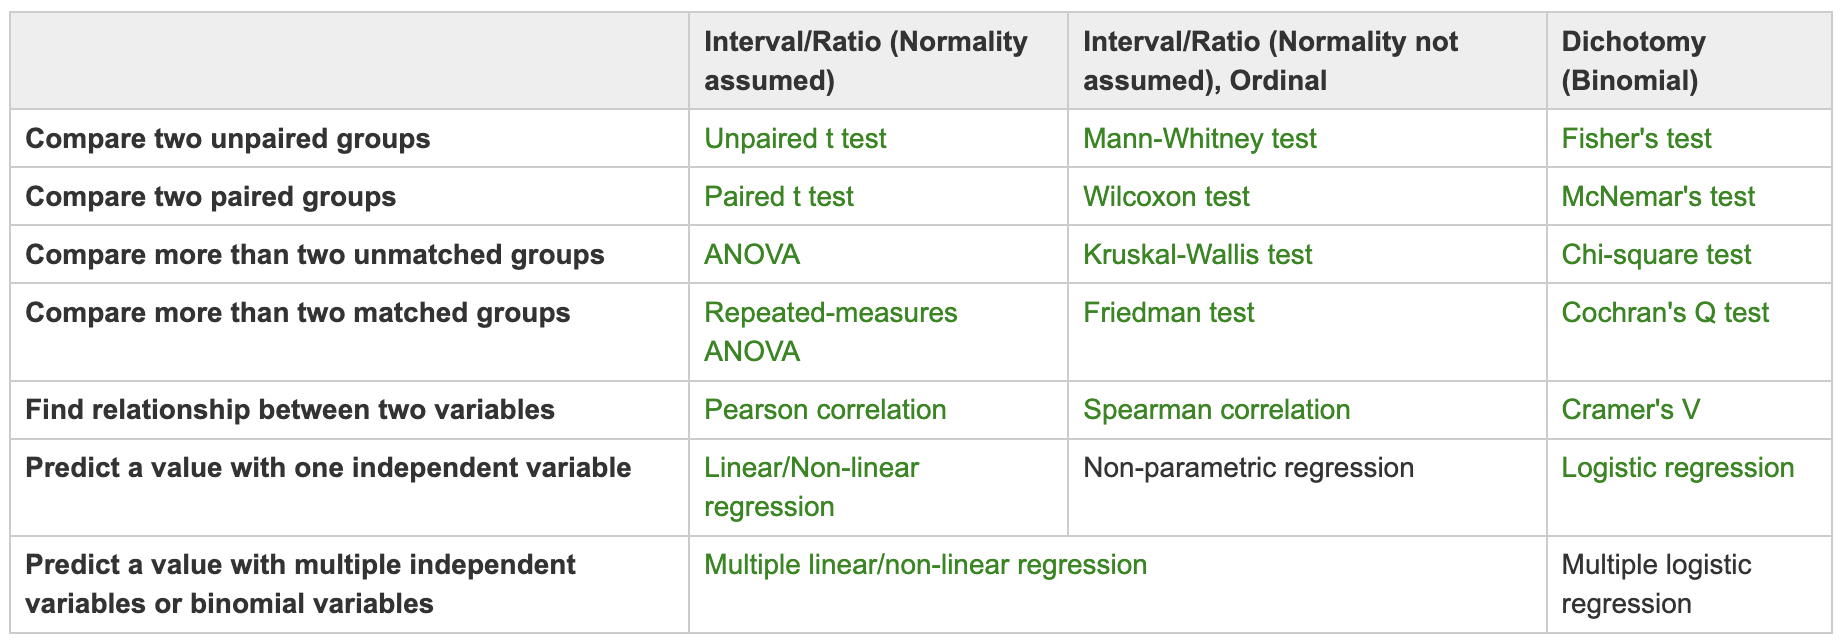
\includegraphics[scale=.25]{lectures/wk10/tests.png}

\subsubsection{Between-subject study: Unpaired vs Paired}
Between-subject study: We cut our participants into 2 groups, which each group trying a different cursors. This is an unpaired group.

If everyone used both cursors, then it matters that these measurements both came from the same person as that would be paired groups.

\subsubsection{t-Test}
1 independent variable with 2 levels,\\
1 dependent variable of type Q (quantitative/interval)

Compares the means of 2 groups\\
Null hypothesis: No difference between means

\myparagraph{Assumptions}
\begin{itemize}
    \item \textbf{Samples are normally distributed}
    \item Very robust in practice
    \item \textbf{Population variances are equal (between subjects tests)}
    \item Reasonably robust for differing variances
    \item \textbf{Individual observations in samples are independent}
\end{itemize}

$t$-Test is somewhat robust to variations in skew as long as the distribution looks somewhat normal.

This is a parametric test.

\subsubsection{Mann-Whitney's U Test}
1 independent variable with 2 levels,\\
1 dependent variable of type O (ordinal), or type Q 
when assumption of normal distribution does not hold.\\
Compares the ranks of values of 2 groups

This is a non-parametric test.

\subsubsection{Parametric vs non-parametric}
t-Tests are parametric as it makes the assumption on the data's distribution (that it is normal). 

Non-parametric test are when one does not rely on a particular distribution.

\myparagraph{When to use non-parametric tests}
Preference data is the most frequently produced ordinal data (Strongly Agree vs Agree vs Neutral vs Disagree vs Strongly Disagree -- so one should use a non-parametric test here).

\subsubsection{ANOVA}
\textbf{Single factor analysis of variance (ANOVA)}:\\
Compare means for 3 or more levels of a single independent variable.

\textbf{Multi-Way Analysis of variance (n-Way ANOVA)}:
Compare more than one independent variable\\
Can find interactions between independent variables

ANOVA tests whether means differ, but does not tell us \textit{which means} differ -- for this we must perform pairwise t-tests.

\subsubsection{Objective measurements}
\begin{itemize}
    \item Good internal validity $\to$ repeatability
    \item \textbf{But, real-world implications may be difficult to foresee\\
Significant results doesn’t imply real-world importance}\\
3.05s versus 3.00s for menu selection
\end{itemize}


    \section{Thursday, March 23rd}
\subsection{Implementing Interfaces, Part 1: Native vs Web Apps}
We have talked about the design process as the cycle that happens in the red phase. In the programming assignments, you have been in the ``Engineering'' phase.

Before we got to GUIs, everyone interacted with computers through command-line prompts, a model where interaction is done via the system.

\subsubsection{Xerox Alto (1973)}
The system is waiting for an interaction and responds once that has happened. This was one of the first interactive programs.

One way you can do this is with a switch statement in an infinite while loop but this only works if your computer is only running 1 process. The reason for this is because they were written by different people.

\subsection{Native Apps: GUI Toolkits}
Today most native apps are written via toolkits such as QT, Cocoa, Java Swing, GTK, etc.

\subsection{Native Apps}
These are self-contained programs made to run directly on a target OS (Windows, Linux, MacOS, Andriod, iOS, etc).

There are a multitude of UI toolkits even if there is a `canonical' toolkit for the OS, and third-party toolkits can help you get closer to the platform-independence that web apps. However this has the cost of not looking like it was \textit{meant} for the current OS.

An advantage of Toolkits over Web Apps is that they are generally quicker in updating to allow using new hardware.

Note that Programming Language is orthogonal to the toolkit. You can use almost any language for almost any toolkit.
\begin{important}
This means that you will have to have an `Android Team' and an `iOS Team' -- even if you share some code, the frontend UI will be split across 2 codebases with completely different code.
\end{important}

\subsubsection{Android SDK Example}
- Highest Level\\
View Class\\
Activity System\\
Native Libraries + Android Runtime\\
Linux Kernel\\
- Lowest Level

\subsection{Web Apps}
This semester we are working on web applications which are delivered by a \textit{web server} and run on a \textit{web browser}.

\begin{shaded}
A \textit{Client} requests resources from  server.
\end{shaded}

\begin{shaded}
A \textit{Server} transfers data for UI and interaction logic to client.
\end{shaded}

\begin{shaded}
A \textit{Browser} on the client parses received data, builds \& renders the UI and processes user input events
\end{shaded}

You can refer to names in the DOM in JavaScript -- a language for defining interactive behavior.

Note that with different OS/vendors, you may see some slight differences.

There are Pros/Cons to using Web \& Native Apps and these can be seen in the table in lecture slides.

\subsection{Disentangling}
We usually separate HTML DSL from CSS/JS code.

Instead of using \texttt{<style>} and \texttt{<script>} tags, we designate explicit \texttt{.css} and \texttt{.js} files for CSS \& JavaSctipt code respectively.

\subsection{DOM (Document Object Model)}
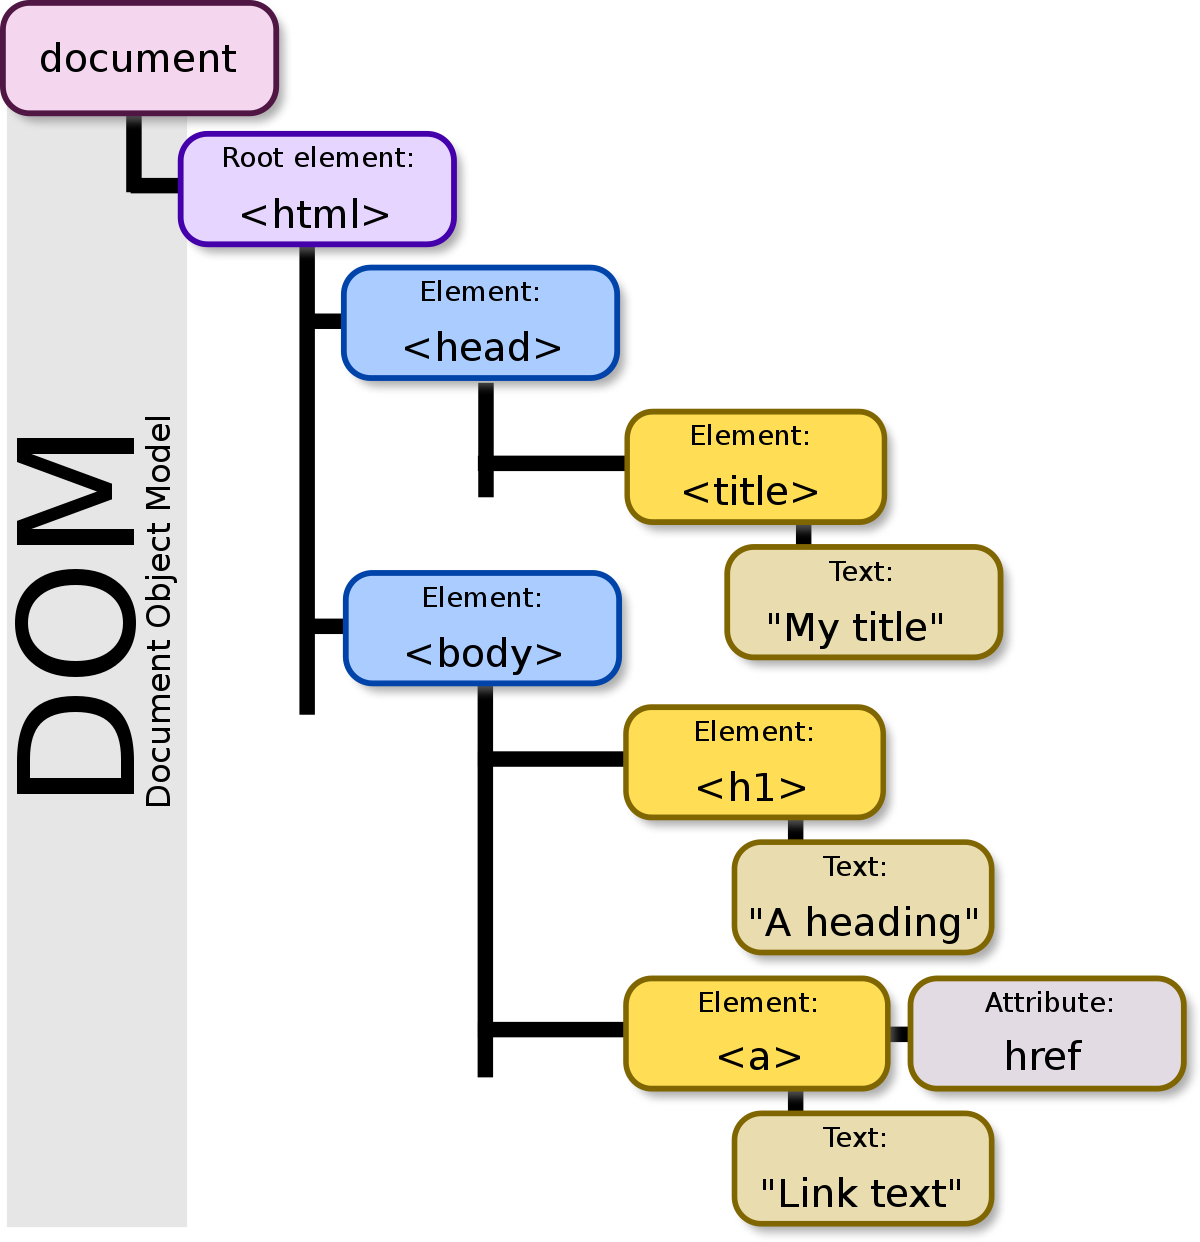
\includegraphics[scale=0.15]{lectures/wk10/dom.png}

\subsection{Web App with server-side code}
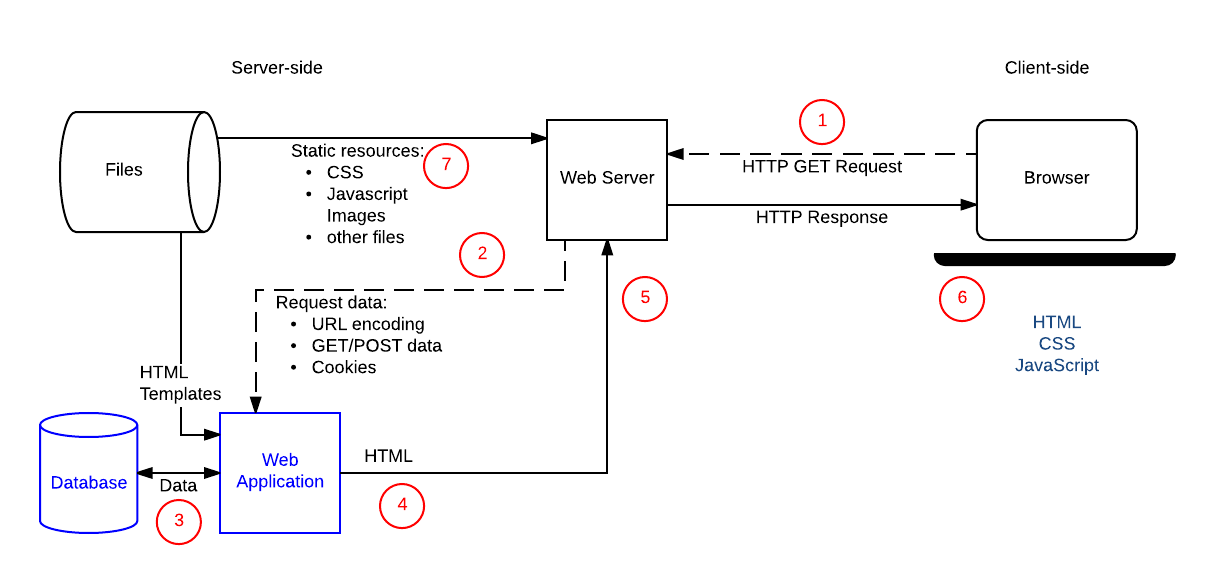
\includegraphics[scale=0.75]{lectures/wk10/web_app.png}


\subsection{Client-side Web Frameworks}
HTML was made for \textit{Documents} -- not UI.
\begin{itemize}
    \item React JS (Facebook)
    \item Angular JS (Google)
    \item JQuery
\end{itemize}
Note that JQuery is still considered a Client-side Web Framework even though it does not really change how your server communicates like the others.


    \section{Tuesday, April 4th}
\subsection{Unexpected Circumstances}
The Professor tested positive for COVID, and thus class will be virtual for today and Thursday.

\subsection{Administrative Matters}
Midterm 1 grades have been released. The midterm was out of 125 points total (though there were up to five extra credit points). The following statistics are about normal for an exam in CS 160.
\begin{center}
    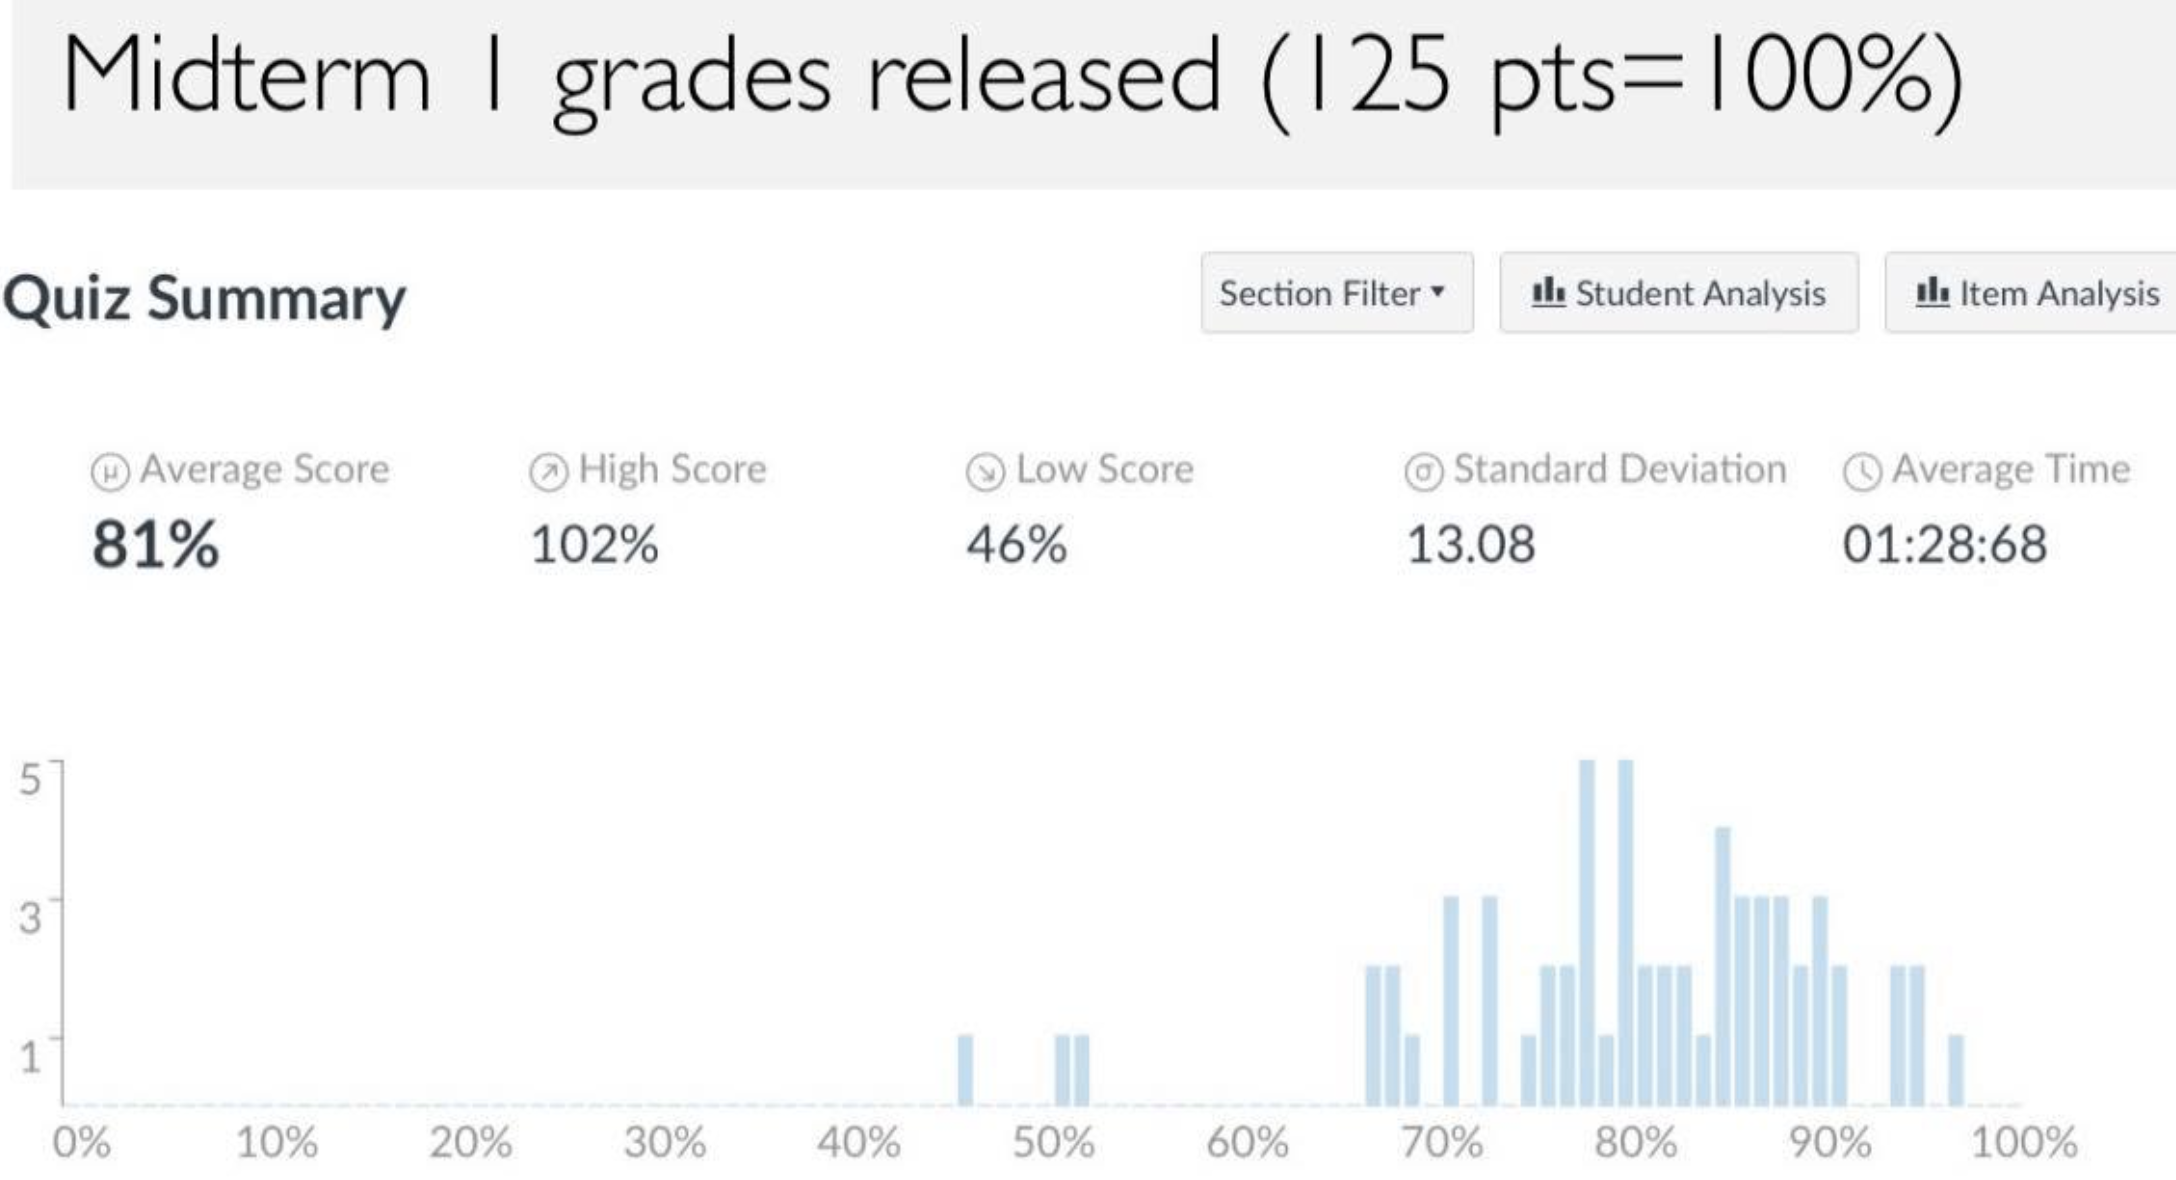
\includegraphics[scale=0.25]
    {lectures/wk11/img/midterm_grades.png}
\end{center}

\subsubsection{Midterm 1 Regrades}
Standard regrade policy applies here to request a regrade, please write a detailed explanation for your request and submitted via the regrade request form that's on the syllabus for the course. Please do that within one week. Do not email directly -- then Course Staff just lose track of all the requests. Make sure to do this especially if the point total on the question does not match the feedback you've been given. Or if we just forgot this to grade something, we're fallible, this happens, sorry, we will fix that. Please do not argue with us about partial credit. Credit on a given question. Since like one person consistently graded a poll question for everyone in the class. And so we tried to be very consistent in how we assign partial credit. So your number is in similar in relation to other students who provided a similar answer. 

\subsubsection{Midterm 2 Logistics}
Midterm \#2 will take place next week, Tuesday April 11th 2023. 

The format will be the same as midterm \#1 -- it will be released the midterm online through bcourses at 09:00 A.M. 

You will have 90 min within a 24-hour time, 24 hour time window to take the exam which will once again have a mix of multiple choice and open answer questions. 
\begin{important}
Midterm \#2 is not cumulative. This is \textbf{not} a final exam. We will only ask about material that was not yet covered in midterm \#1. 
\end{important}

\subsubsection{Scope:}
\begin{shaded}
This means the material we'll cover is that from lectures 14 through 20, information visualization, usability inspection methods, usability evaluation, data analysis, and three lectures on implementation of which we are in the second right now. 
\end{shaded}

\myparagraph{Readings Scope}
Readings: we will not ask you about information visualization readings since we made that optional. We will ask you about the two Martin chapters on experiment design interpreting data. The heuristic evaluation links provided in the heuristic evaluation assignment are also fair game -- they should pretty much match what we covered in class. The last reading on how browsers work is also in-scope.

\myparagraph{Course curving scheme}
Question: Is this class curved?\\
Answer: This class is not usually curved. Usually we get just about what we want in terms of a an upper division or a master's class great distribution by just taking straight values. Usually the exams tend to be a little lower than the project assignments and the homework assignment grades. We will definitely not curved down. We can take a look if all the values are significantly below where they should be. If so, then we curve up but haven't had to do that in the past -- so I would not expect that to happen this year either. 

\subsubsection{Next Team Project Assignment}
The next team project assignment is a heuristic evaluation. Now, heuristic evaluation is a discount usability method as we discussed, that should be quick to do. That's why we only were only assigning one week. And in fact, you will do most of the work for this assignment. In section this week. You will conduct a heuristic evaluation on another team's Figma prototype and vice versa. Another team will evaluate your Figma prototype. This will happen in sections, so it's important to attend section. You will then share the report of what juristic violations you found with the other team within 24 h of section. And you will receive your report and then you as a team, we'll discuss, well, what should we do, what should we redesign based on these usability violations that were found? Briefly write that up, and then submit that to us. So I would say the majority of the work for this assignment happens in section. And then maybe there's another hour or so a team meeting that you should have afterwards to interpret the results. So in the larger scheme of things, this is a much smaller team assignment than the ones you've done previously. If since you submitted your Figma prototypes to us, you've had other ideas, your thinking has evolved. Feel free to iterate and change your Figma prototype. Before this week's section. If you think it's fine, you don't need to do anything. \\
Following this week, we will have three weeks of weekly implementation check-ins in sections. So you will submit a brief progress updates to us. And then in section, meet with your team to work on your project and also check in with your GSI to discuss your progress, what you've accomplished, what remains to be done, what your plan is. So we want you to every week for the following three weeks basically make for here on progress. So you're not keeping it all for a rush at the end. That takes us through the last week of regular classes. During RRR week. We then have our scheduled demo session, that is Wednesday, May 3rd at 02:00 P.M. That's where we will you will show your final demo to class staff and the public. And you will also have a poster about your project. And then during finals week, one week afterwards, we give you one extra week to put together final video and team evaluation. 

\subsection{Native App Concepts}
\begin{itemize}
    \item Native applications provide a “cleaner” and simpler architecture for constructing interactive applications bc that SW stack was built for interactivity
    \item Web apps had interactivity added on top of a document-centric, distributed client-server system
    \item GUI Toolkits
    \begin{itemize}
        \item We don't write the main function
    \end{itemize}

    \item Widgets
    \begin{itemize}
        \item Modular components that get reused again and again
        \item Ex. Android lists or date/time pickers, buttons, toggles, text fields, etc
    \end{itemize}
    
    \item UI Components
    \begin{itemize}
        \item Each component is an object with:
            \begin{itemize}
                \item Bounding box
                \item Paint method for drawing itself
                \item Something else
            \end{itemize}
        \item 2D graphics model
            \begin{itemize}
                \item Typically top left to bottom right
            \end{itemize}
        \item Sizing
        \begin{itemize}
            \item Widgets are not in control, bounding box is controlled by Layout Manager
            \item Component has to know how to draw itself at a size provided by LM
        \end{itemize}
    \end{itemize}
    
    \item Working with Widgets
    \begin{itemize}
        \item Make common case fast, uncommon case possible
        \item Common case: assemble standard widgets into a layout
        \begin{itemize}
            \item Instantiate class, provide configuration parameters
        \end{itemize}
    
        \item Uncommon case: write your own widget
    \end{itemize}
    
    \item Absolute layout
    \begin{itemize}
        \item Good idea? Provide absolute coordinates for everything
        \begin{itemize}
            \item Bad idea in general outside of prototyping, hardcoding parameters only works for a given screen size
        \end{itemize}
    \end{itemize}
    
    \item Event Dispatch Loop
    \begin{itemize}
        \item Mouse moved = Event Queue (sorted queue of input events) → Event Loop (runs in dedicated thread)
        \begin{itemize}
            \item Event Loop:
            \begin{itemize}
                \item Remove next event from queue
                \item Determine event type
                \item Find proper components
                \item Invoke callbacks on components
                \item Repeat or wait until event arrives
            \end{itemize}
        \end{itemize}
        
        \item $\to$ Component (invoked callback method, update application state, request repaint if needed)
    
        \item Model-View-Controller
        \begin{itemize}
            \item Model
            \item View
            \item Controller
            \begin{itemize}
                \item Receives input events from user, decides what to do by talking to view to determine which objects are being manipulated
                \item Calls model methods to make changes on objects
                \item Model then notifies views to change
            \end{itemize}
        \end{itemize}
    
        \item Why MVC?
        \begin{itemize}
            \item Combining MVC into one class will not scale
        \end{itemize}
    \end{itemize}
\end{itemize}

    \section{Thursday, April 6th}
\subsection{Midterm Logistics Review}
This is the last class before our next midterm -- so we will start by reviewing the midterm info again: Midterm \#2 is next Tuesday, April 11th. The same format as midterm number one, which means you don't have to come to the classroom. You can if you want, but the midterm is happening online, will release it at 09:00 A.M. you then have 90 min or 90 min times here DSP exam time within a 24 hour window to take the exam. It is on bcourses as a quiz. We once again have a mix of multiple choice and open answer questions. Most importantly, it is not cumulative. Only material that's not been covered in midterm, one will be on the midterm too. So what is that material? Well, it's lectures 14 through 20, information visualization through number 20, that's today, browsers. And the associated readings, which include the two readings, experiment design and interpreting data. The readings on heuristic evaluation, which will lengthen your heuristic evaluation assignment and then how browsers work. Reading that we assigned. You don't have to submit an answer, but it's a part of it. 

We had some questions about practice midterms. So there are two practice midterms on bcourses under Files, midterms. Those were both examples of second midterms from CS 160. And just the caveat, that material has slightly changed. So we will not ask you about the specifics of Android. You might see some questions in the practice midterms about that because that is no longer the focus of the class. We will also not ask you about midterm one material. So some of the practice midterms, e.g. have questions about color spaces, which we already covered in midterm. Number one. So take it as a guideline of the types of questions we'll ask, the format of the, of the questions, but we will tailor it to the actual lectures we covered this semester. It will once again be open book, open notes, but you shouldn't be talking to other students in the class about the exam, just like midterm number one question, will there be coding? We might ask you some questions that where we show you some code and ask questions about it. Like we might show you HTML, CSS, and JavaScript, but we will not ask you to write code. Yeah, So just to repeat, we might show you code, but we don't ask you to write code to answer the questions. 
\subsection{Implementation}
Today will probably be a shorter lecture partially because it's such a complex topic -- and we should just focus on the the high-level takeaways.

\subsection{Where are we in the course?}
We talked a lot about the design phase and right now we're in the kind of what's the engineering of user interfaces look like. That's what you're programming assignments were about, that's what your implementation of your team project is about. And then in the lectures that we're currently having, we're looking like one layer beyond that because the code you write, What's the system underneath it that works with that code to actually render interactive interfaces to the user. Okay, so here's the quick review of what we talked about last lecture. So native application concepts, right? What did we talk about? We talked about key concepts or widgets or controls. Those are the templates for buttons, date pickers, drop-down menus, radio buttons, etc. And how are they architected? Well, they implement drawing, bounds management and event processing. So they know how to draw themselves. They know how to draw themselves when they get resized. And they can process input events. And some of that processing comes kinda out of the box, right? So a button automatically renders itself as depressed when you press the mouse button over it. And then some of the event processing is basically gives the structure for you to add your own code. So your event handlers so that your own code can execute when that button gets pressed by the user. We talked about that widgets are laid out in a containment hierarchy, right? So we have this tree where all the internal nodes of the tree, our layout nodes and all the leaf nodes are the actual widgets. And the layouts determine how the children of the layout note get arranged on screen. And so parents allocate space for children. And so the layouts allocate space and then tell the widgets, Hey, you have the following bounds. Draw yourself. We've talked about most modern UI toolkits support declarative layout of UIs. So basically, this is usually done in some XML dialect. Right here. What happens in native apps looks kind of like what happens in HTML. You have some XML dialect that specifies at compile time what the structure of the Uighurs. 

However, we also want this to be flexible. And so usually they're also, you can encode also directly manipulate that, that structure to dynamically change the tree at runtime. Then we also talked about events. And events are how we deliver information about user input. Two components and the user interface. And they are the key diagram we talked about was the event dispatch loop, right? Where you have a Q input events go into that queue. The main event loop in your UI toolkit pops these events off one-by-one, figures out what UI components to deliver them too, and then calls the appropriate event handlers on those UI components and delivers the event to them. Then the last thing we talked about was Model-View-Controller. As a way when you do object oriented programming, how do you write the classes that make up a user interface in a way that is extensible and maintainable. And so the key concepts there's you have model classes that just capture all of the information, right? So in a drawing app that would be describe the shapes that are on screen. How big are they? What are their positions? What are their colors and other attributes? Then we have the view classes, which are responsible for rendering a model onto screen. And then we have the controller classes which take input from an input device and then update the model. Then when the model updates, right, the associated views update. And so that was the cycle of how we go from input to output. But in a structured way that is easily extensible and maintainable. So we can add information to our model without having to touch any of the view code. We can add extra views to our application without touching any of the model code. All right? 

Here are a couple of things we already talked about. Event handling, part of the model or controller. So great question. Event handling is not part of the model. It's part of the controller. The controller receives the input, such as I drag on the handle of a shape that's onscreen. The controller may then interpret this as 0. That means I should the user just re-size this shape. So let me find the model class and update its internal width parameter, which in turn then leads to a request to redraw the screen. But event handling happens in the controller. But as a result, we usually then in the controller update the model. Another way to think about this is that if you're assembling your UI from pre-existing widgets and controls, right? Event handling happens in Callback functions on that, on that widget. So that's a control class. Usually you're the internal, how you store information about the application. Those are classes that you create that are not subclasses of widgets and controls, right? Those are model classes. And so event handling happens in the controller, but it often updates a model class as a result. Okay? And then I wanted to go over these slides again. So we talked about wet versus native apps, some pros and cons when you would choose which makes a compatibility on the web is great. You need one code base. We're native apps, it's platform specific, and you might need multiple code bases if you target multiple mobile or laptop operating systems. Software updates and web apps are of course, incident. As soon as you push new code to the server on native apps, that requires we installation of the application. But web apps by themselves cannot run offline. Native apps can. However, these days can all the data usually involves some web service. And so even a native app. What good is Netflix? If you can start up the Netflix app, but you can't access any movies. Not that useful. In terms of functionality we talked about that web apps are often kind of one generation behind what is available natively. And that when a new piece of hardware comes, comes around, like a depth camera or another new type of sensor. That usually, there's usually a native application framework first for using making, taking advantage of that hardware. And then performance-wise, usually web apps have lower performance because there's the additional complexity of the browser and we tackle some of that complexity today. Whereas the native applications you can write. Timing critical components in some low-level compile fast language. And then we also did some mapping of concepts onto each other, right? So how do you declaratively define what the UI structure look likes? It looks like in a native app that some XML layout file in the web app. It's HTML. And we'll talk again how today, how that is not a true XML file, even though it looks like one. Visual appearance rules, we use CSS and Web Apps. And there's usually a notion of styles and themes and Android or other native apps. Css is an especially complex way of implementing visual appearance rules. We'll talk about that a little bit today as well. Application logic is usually written in some native language, right? And UI toolkit in a native application, in a web app gets split across client and server. 

We usually have some way of bridging between the application logic and that declarative UI structure. And how do you define different screens? Well, in a native application that is usually some class, whereas in a web app is just you navigate to a new URL. One last piece of review is what happens when we request a web page from a server. So basically this is the quick review of how do we get all the HTML, CSS, and JavaScript to the browser? And then the rest of today's lecture is, once it's in the browser, what do we do with it? So remember that for web apps, we need a web server. The web server has access to files and then our computer, the computer of the user in this case is the client. It sends a request for a particular resource to a web server. So that happens for web apps over HTTP, Hypertext Transfer Protocol Addresses are encoded as URLs, Uniform Resource Locators. The web server receives the request and then maps that through its internal logic to, okay, so what files do I need to retrieve from my file system? What HTML, CSS, JavaScript should I retrieve? It can of course construct these on the fly as well with computation. It then delivers them back to client and the client. The browser then renders the files as a web app user interface. All right, so then today, the topic is once we've received those types of files like HTTP or HTTPS and the browser, what happens next? And so I'm just going to walk through some of the key concepts in the reading that I've assigned for this. Alright, high-level structure of the browser. The browser's main components are the user interface of the browser as well itself. That is, everything that's not the browser window, right? It is the menu bar. For the browser. It is the URL bar where you enter the URL. It's the backwards button, it's the bookmarks, etc. So everything that's not the requested page itself. Then there's a pair of a browser and a rendering engine. The rendering engine is the key most complex component for displaying the requested content. So if you request it an HTML document, it's responsible for parsing the HTML and the CSS and displaying that on screen. We will mostly talk about that today. The browser engine is basically the layer in-between. Like that, uses what you do in the browser user interface to send commands to the rendering engine. There's a networking component, which is basically the previous three slides, right? How do we actually get the documents from the network for requested URL? And then for all the other documents that might be LinkedIn, it is a JavaScript interpreter, which is usually separate from the rendering engine. So here's a difference between native apps and web apps. And native apps were the Part of interpreting the UI and where you put the callbacks, that's part of the same UI toolkit in the browser, we have separate render, rendering engines of JavaScript interpreter's. The browser also then has a UI backend. We're basically says, Okay, I've received all of this HTML and CSS. When it comes time to draw it on the screen, it's still uses the underlying graphics primitives of the platform it's running on. So just like a UI toolkit in the end will resort to 2D drawing primitives like put text on the screen here, draw a line, draw a rectangle. The browser in the end uses those same calls as well. Then the last component is there's usually a data persistence layer where e.g. all the cookies that you receive gets stored. And HTML5 also has kind of a local storage component where data that's local to the user can be stored in the browser. 

All right, So that's the high-level structure of the different components of a browser. And then most of today we're going to spend on an overview of how rendering and JavaScript works. So, okay, question here was, what about the direct arrow from user-interface to UI backend? When does this happen? So think about the browser Chrome, like thinking about the address bar and the back button in the browser, that has to get drawn on screen as well, right? And so there, the user interface component of the browser uses the UI backend to use those low-level drawing primitives to put the buttons and menus on screen. Thanks for the question. All right, let's keep going here. Okay. So high-level overview, what the rendering engine does, it is it gets the HTML and the CSS. It has to parse them to understand their structure. So HTML goes kind of video content tree, CSS goes into a style tree, and then that information has to be fused together to determine for a given element what style should we render it in? That's called constructing the render tree. And then the render tree has all of the components that should be displayed on screen and now has their visual styles. And then there's a layout pass where you determine, well, where, how big is it, where should it go on screen? And then once you've done a passive or that, then painting happens, which is using the UI backend. You just draw stuff into the viewport. On the JavaScript engine, we get the JavaScript, we parse that, we compile it and execute it. Alright, so let's delve into that. Let's start with the rendering engine. Okay? So the rendering engine, that's the piece of code that's responsible for displaying the received content in the browser window. Most of the code and rendering engines focus on HTML CSS, because that is what the width is built on. But rendering engines can also have plug-ins and extensions to handle other formats, right? E.g. most browsers can directly render a PDF. So there are some extension for rendering PDF structured data. But most of the core of the rendering engine is for HTML and CSS. Now, different browsers use different engines. And one thing that's interesting here is that basically what we use today is all, all goes back to open source software. So for those of you who are using Linux, you might have at some point used browser called Katie conqueror. And that had a rendering engine called K. Html was particularly standards compliant. And then pretty much everything else that the commercial companies use these days somehow goes back to that open source code base. So Apple Safari browser, the rendering engine is called webkit and web kit at some point was forked from K HTML. Google Chrome uses a rendering engine called blink. Blink at some point was forked from webkit, or more precisely, it's web core component. So also goes back to HTML. Interesting detail is if you use Chrome on iOS, on an iPhone, then it actually Doesn't use blink, it uses webkit because that's an App Store policy in iOS. So their Chrome actually uses different rendering engines based on the platform that you use it on. Microsoft Edge, microsoft used to use it, right, its own rendering engine. They've now abandoned that and they're also using blink. And then the only other kind of independent project that has significant traction is Mozilla Firefox. They use gecko and of course, Firefox also open-source project. Let's look in one level more detail how this rendering engine flow works. So we start by receiving HTML and style sheets. Then we parse the HTML and the output of that is a DOM tree. 

So the Document Object Model tree, style sheets, we parsed and we get a tree of style rules. And then there's this merging process where we attach style rules to particular elements in the DOM. And that yields a render tree. The render tree has to go through a layout phase and then goes to painting to draw. Once layout determines the sizes and positions of elements, we painted onto screen, onto the display. 

\subsection{Parsers}
Alright, so let's talk for a minute here about parsers, how that works. So let's maybe get a show of hands. 
\begin{shaded}
Who here has taken CS 164 or a version of it -- a PL (Programming Languages) course.
\end{shaded}
Today we are gonna to see the high level intuition of how basically HTML and CSS are custom domain specific languages that for you to program a document structure and visual attributes. And here's like one-six-four in a nutshell of how you parse and then interpret a custom domain specific language. If you want to know more about it than I highly recommend you take that course probably with Sarah Jason's or Zen. Super important can a basic topic in computer science. Okay? So we just received a document which is basically a bunch of characters and we want to understand the meaning of that document. So a common pattern, Which mode, which we use to interpret most programming languages and most domain-specific languages is. We go through a two-step process of first flexing and then parsing. And so lexical analysis, we usually, we turn the document that we've received into a stream of tokens. And so a token could be, this is a string, this is a number. This is a special character. Usually we define what a token is, two regular expressions. So we passed all the characters we received in a document through a set of regular expressions. See which ones match, and then emit a bunch of tokens. In the next step, we then consume the stream of tokens and try to build a hierarchical representation. So a parse tree out of this tokens. The way we use that we do that is usually we define a context-free grammar that defines the structure of legal statements and expressions in our language. The usual tools that you, there's lots of tooling around that. And so traditionally in Unix and used to be lex and yacc, those tools are now called flex and bison. So one is a lexer, the other one is a parser. There's also, by Professor at the University of San Francisco, wrote a tool that has a great community called antler, which is a parser generator. And so what you usually do is you provide a definition of for Alexa, you provide a definition for a parser. And then a parser generator will generate the code that can then process a document and give you a parse tree back. So let's look at a really simple example. Let's look at here's a snippet of valid XML. Tag, attribute equals value, some text in between and then end tag. How do we create a parse tree for that example? So here's what a simplified XML lexer and Parser would look like. That could deal with such input. So first you would define a lexer. So here what you see is basically on the left-hand side, you see a definition like I define a token like tags start open. That's the name of my token. And what is it? Well, it's the string Open tag. Tag closes the string close tag. Then we have something like a digit. And now this is a regular expression. It's a digit 0-9. Letter is between lowercase a to lowercase z or uppercase a through uppercase Z. Whitespace is a tab. New line or a space. I'm an identifier is a letter or some sequence of letters and digits, right? So I define a bunch of regular expressions and give them names. And once I have these in place, right, I can just scan like start scanning the text I'm given and say, Oh, here's a tag, start open. So I admit that I emit that token, does. Next thing that matches what I defined as generic ID is another generic idea. Here's a tag close. Here's something that's not within a tag in in XML that's called PC data. Parsed character data, sorry. And so we just turn this document we received into a set of tokens. And then the next thing you do is once I have that set of tokens, I define a grammar. Where the grammar can have I defined rules that match some sequence of tokens and other rules, right? So e.g. two, start, the start tag in XML. Is we have that. Sorry, let me try to get to. This is just this character, right? Generic ID, that is the name of the tag. Then we close the tag, that is this. And then we have zero or more attributes that can be in there. What's an attribute? Well, this is a different rule. An attribute has some name, equals, that's the equal sign. And then it has a value. And then by the end, so we define these rules. And then we say an element in XML has a start tag. Inside of it. It can either have other elements or just some texts. Zero more of those. And then we have an end tag. So now we've defined a grammar over these tokens. And what I can now then do is construct a tree based on matching grammar rules, right? So we have a top-end element that is this whole string. Within that. We have start tag that goes from here to here. We have some text inside of it that is from here to here. We have N tag that goes from here to here. And then within the star tag, this matches the name of the tag itself. And then we have an attribute node, which has an ID, which is this part, and a value which is this part. Of course, inside of this tag, we might have other tags in here, right? And then the tree would just get more complex. So through this two-state stage process, we started off with just some character data that we received in the browser. And then we now turned it into a scree representation of that domain specific language. Okay? So unfortunately that is, it would be great if we, we're done here. That's the basic approach of how you parse CSS and JavaScript. For both CSS and JavaScript. We can define a set of lexer rules. We can define a context-free grammar and we can parse it in that form. Unfortunately, that does not work for HTML. And other question is, why not? Html looks like XML, right? Shouldn't just be an XML dialect. And unfortunately, HTML rakes some of the rules of XML in a couple of ways. So examples of valid HTML that are not valid XML, an image tag, the image source URL here. Why is this not valid XML? Because it doesn't add any point have a closing tag. Same thing for a new line, a line break. What's missing? We don't have a closing tag. Another example, you can write input type equals checkbox. But based on the rules that we defined, every attribute, the value has to be in quotes. So there's a bunch of ways in which you can write HTML that's valid HTML. But it's not valid XML. As a result, you cannot use standard context-free grammar based parser. It can deal with these edge cases. The other big reason is lots of people write HTML by hand and they make a bunch of mistakes. And browsers want to be able to render HTML even in the presence of errors. They don't just want to throw up an error set malformed HTML. I'm not going to show you anything. Let's talk about that for a moment. Okay, here's some HTML. Look at it and tell me in the chat what is wrong with the following snippet of HTML? There are multiple errors in here. Look at it, think about it, and then tell me in the chat what you think is wrong. Alright? Says nested tags. In particular, what's, what's wrong with the nesting? Yeah, okay, farm Rahul and rationality all have the right idea, right? As these two go together. And these two go together. This breaks the nesting relationship. The P has to be closed within the div to be valid, right? But people do this, people write stuff like this. So the p, This would need to move down here. Okay. Anything else you see that is wrong, right? My tag that doesn't exist, that is not a valid HTML tag, not part of the HTML spec. So what should a browser do when it receives such HTML? To just throw basically a compile-time error was like, I'm not going to render this document. In general, browsers say no, that's not what we should do. We should try to fix the errors that are here and just do a best effort at rendering. 

Okay? So what happens is HTML parsers as implemented in browsers, they still have a tokenization and a tree construction phase. But we don't just use the standard lexer and a parser. There's like more complicated code that runs that e.g. checks for all kinds of custom error conditions and then corrects the HTML's ago, we think maybe you meant this. So we're not gonna go into the details of how that happens, but you can look it up into HTML spec on this link, which suggests the structure of such a parser. So high-level structure of the parts are still the same, but at a low-level would actually happens under the hood is way more complex. Okay. Now we get to parceling CSS. Css is much more well-behaved. Css. The language definition for CSS is really clean and can be parsed with the standard lexer and Parser. So we take something like the character stream up here and then we produce a tree of CSS. Alright, so we've passed our HTML with a much more complex parser, constructed a DOM. We parsed CSS and we now have our CSS tree. What do we need to do next? Well, what we want to end up with is a render tree. So a render tree has the visual elements in the order they will be displayed on the page. And each node or render knows how to layout itself and its children. So that's a render tree, kind of like containment hierarchy, right? Each node knows how to draw itself. The renderers and the render tree kind of correspond to DOM elements, but the relationship is not one-to-one. E.g. the head element in HTML, anything that's in the head doesn't get rendered in the viewport. Elements with a CSS style of display, none are not rendered. On the other hand, we have complex elements like a drop-down on a form that might need multiple renderers. So we end up with some tree here that has a relationship to the DOM, but it's not necessarily a one-to-one relationship. The next important thing we need to do is we need to match which visual styles that are defined in CSS and HTML we should attach to each of the nodes in our render tree. Visual styles. There's a bunch of different ways in which you can define visual styles. So you can author CSS rules. Css document. You can also in the HTML L itself, have CSS style attributes. In addition, HTML has visual attributes, like setting the background color on a paragraph, which is not CSS syntax, but also defines a visual style. We have three different sources of where style rules come from. And then for the CSS rules, they actually can be many different style sheets that a single UI loads it. So in particular, there are not just the page style sheets. These are the ones that as an application developer, you define. But the browser also has a default style sheets. So if there are no CSS rules, what font you use, how big should it be? That's a browser default style sheet. And then each user profile in the browser can also have style sheets where you just set your preferences. I want everything rendered at 150 per cent. I prefer the following background. And then each style sheet can have many rules. Now there's a question of, well, how do we look up which rule to apply when this is where the cascade order comes in, which is the C in CSS, right there. Not just style sheets, but they are cascading style sheets. So what does the cascade order mean? You can look it up in the specification for CSS. It basically says there is an important, there's an order of importance. So in ascending order, the least important rules are user agent that those are the browser rules. Browser user normal declarations, these are the user's preferences. Author declarations are the author of the web app, right? So this is web app. And then there is a level of importance. So if you have a exclamation mark important rule, then it kinda supersedes others. So you first look up, is there a user important declaration? If not, let's go through the Web App declarations. Then let's go through the user's normal preferences and then the browser preferences. And basically the higher, the higher ones take precedence over the low ones. So that's what we mean by the cascade order in cascading style sheets. And then the other part that happens is we have a tree, right? We have a tree of HTML. Elements are dumb. Next thing that happens, let's say we're at this element down here. What do we do? We look up the cascade. So these were the rules I just talked about. Can we find a value for background or text color? If so, we use it. If not, we go up the tree and we check, did this node define background, color and font? If so, we use it from here. If not, we go yet further up the tree. So the upshot of all of that is actually matching styles two nodes is not a trivial process at all. You need to consider multiple sources and different preferences, which makes the whole thing kind of more complex than if you just have a style parameter in a native UI. Alright? But at the end of this render tree construction, we basically have everything that gets rendered on onscreen and we have the right CSS style attributes attached to each of the nodes. The final thing we have to do is now we have the styles, but we don't yet have the sizes. And so the final path that happens is a layout stage, where we basically go from Herron down the tree to children. We determine the width of an element that could come e.g. from a CSS style rule. Then we recurse on the children, call land on the children if needed. Maybe calculate their height and then from all of those heights, we calculate our own heights. So it's kind of a panel down, bubble up algorithm where based on available width, the calculate heights, and set those for the whole tree. And then we have basically the bounds for each of the boxes. And once we have those box bounds, we can just call paint. And then paint. It now has all of the absolute coordinates that it should use and abuse this drawing primitives like put texts at x location x, y with the following color and the following font. But this is now this uses the same underlying primitives as UI toolkit in its draw method. So we have access to 2D drawing primitives, lines, boxes, texts, colors. So one way to look at it is that this whole rendering engine, I'm in the browser does the work of the UI toolkit. It just does it in a kind of a more complex way because we have to deal with the vagaries of HTML. We have to be very error permissive. Whereas a UI toolkit, if you give it a malformed XML, let's say error can't deal with this. And on the other hand, we have this really flexible Cascading Style System, which is also more complex than style definitions in native UI Toolkit. Okay, then just briefly, so we just covered what is happening up here. And then just briefly wanted to touch on what's happening down here, but not in a lot of detail. Which is we also get a bunch of JavaScript from the web server, right? So what do we do with that? So the first part is we parse it. So a JavaScript parser. This here is kind of what we just talked about in the parsing S aspects. So we'll have a lexer and a parser. And then in the end, we end up with an abstract syntax tree, which is a tree presentation of the code we just received. Now, JavaScript is an interpreted language. But interpreting all of the JavaScript that we received would be too slow. That's what web browsers did in the very early days of the web. This is not what we do any anymore. Instead, we compile JavaScript using a just-in-time or a JIT compiler into machine code. And then. Execute that to speed it up. And in fact, just this box of how do we make JavaScript faster has been endless engineering on that part. And what's actually happening in browsers these days under the hood is not just we don't interpret, but it's more complex than that. So here e.g. is an example of what the V8 JavaScript engine does in Chrome. And it basically has two pathways. He has a compiler that this is the fast pass. So we get our source code, we compile it into bytecode. We have a bytecode interpreter and executed. And while this execution is happening, if we have spare cycles, will say, Well, we tried to go through this path as fast as possible. But as a result, this is not highly optimized. It's way better than interpreting it, but it's still kinda slow. So that's in the background. Launch another path. And try to optimize this bytecode that we received with an optimizing compiler. And once that is ready, replace this binary with an optimized binary and start executing that. Kinda way more complex. Again, then what's happening in a UI toolkit, right? We're, we're just, we're compiling the code that you gave us and we're running it at runtime. Based on the design decisions that were made early on is that we attach this JavaScript. We're just kind of by accident, this interpreted language took over. And now we have to deal with the fact that we have this kind of not very optimal language. But we really want fast application performance. And so we need way more machinery on the backend to get something like native performance out of it. Okay, so there are tons of details like if you want to become a browser engineer. So Irina asks, I'm curious why not just do the optimization first, then render the optimized code. Because this path down here is fast to compute. Slow to execute. This path up here is slow to compute and then passed to execute. 

So the desire is that like your web browser is loading and this JavaScript code, we want to start executing it as quickly as possible, right? So from the time, from the time that we receive this document of JavaScript, we want to start executing that code right away. So you want to do the fast just-in-time compilation and start executing it. Then in the background, say, well, yeah, but now this execution, this bytecode we got, we can probably do better. But it'll take us a couple of hundred milliseconds to maybe optimize it. So we optimize it behind the scenes and then replace it. And yes, either could be faster as the final result. You don't know, right? Because you're just getting this JavaScript code stream then in synchronously in real time. Great question. Okay. That brings us to That's kind of the level at which I want. However this, so if you want to become a browser engineer, that's like being a highly skilled software engineer in all the vagaries of implementing either the rendering engine or the JavaScript engine. I think those are very highly sought after skills, but only a couple of people focused on that. But hopefully, even as a application developer, even if you're never touching the source code of the rendering engine with the JavaScript engine, it's good to have the conceptual overview of what happens underneath the hood and an understanding of it.


    \section{Thursday, April 13th}
\subsection{Collaboration and Social Computing}
\subsubsection{Post Midterm 2 Feedback Form}
Please fill out the form pinned on EdStem if you have anything to share!

\subsection{Remote Communication}
\subsubsection{Zoom}
We all are familiar with online meetings over Zoom.


\subsubsection{Collaboration Apps}
\begin{itemize}
    \item A lot of big companies fell behind because they did not allow for collaboration (ex. Microsoft Word falling behind Google Docs)
    \begin{itemize}
        \item The companies have tried to make up for it (Word now allows collaboration) but it hasn't been enough -- the software wasn't \textbf{designed} for collaboration \textit{from the start}.
        \item This was an easy way to make a lot of money in the early days of (EE)CS -- make a new product which is just an existing product but with collaboration
    \end{itemize}
\end{itemize}

\subsubsection{Calendars}
\begin{shaded}
Who here uses a Google Calendar (or some equivalent) to manage your schedule?
\end{shaded}
As expected, almost everyone in the room raised their hand.

The ability to anonymize what you are doing (and thus not have to worry about people scheduling events they think are `more important' over your existing events) was a key factor in its popularity.


\subsection{Challenges to social software}
\subsubsection{Success crisis:}
\begin{shaded}
    Whether your software scales will only become apparent once you are successful, and then it’s often too late to change the architecture (see Friendster)
\end{shaded}

\subsection{Single Display Groupware}
\subsubsection{Roomware}
Example: AT\&T Network Center Control Room -- has everyone in the same room at the same time, even if they have different responsibilities. This helps develop a shared sense of purpose for the end-goal and allows people to be up to the date wth the overall project status.

\subsection{Graph Theory}
\begin{itemize}
    \item  \# of edges in a fully connected graph: $n*(n-1)/2 \quad\sim n^2$
    \item \# of edges in a tree: $n-1$
\end{itemize}

\begin{shaded}
    \textbf{Coasean Floor}: The point below which the transaction costs of a particular type of activity are too high for a standard institution to pursue.
    $\hfill\text{- Clay Shirky}$
\end{shaded}

\subsection{Power Law Distributions}
\begin{center}
    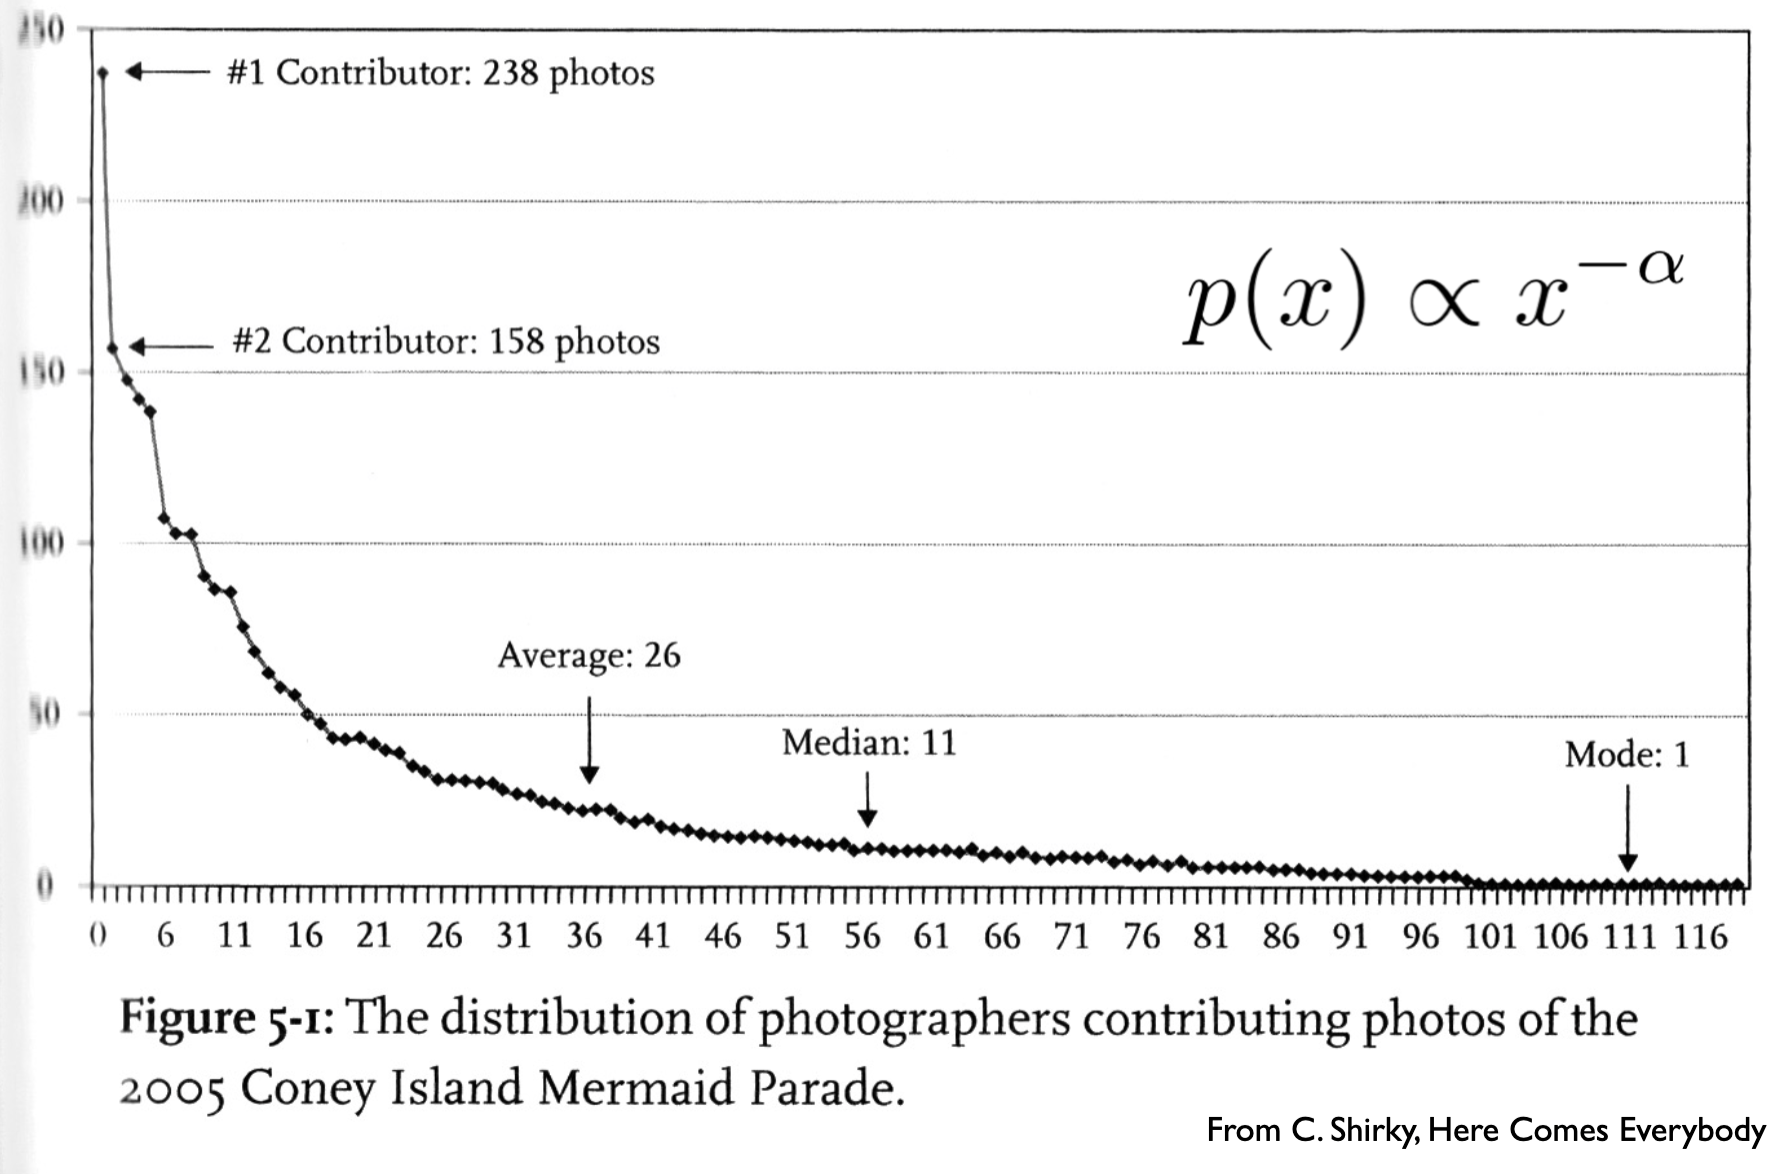
\includegraphics[scale=0.5]{lectures/wk12/img/pl_distro.png}
\end{center}
\[
p(x)\propto x^{-\alpha}
\]

\subsection{Time/Space Matrix}
\begin{tabular}{ |s|l|l| }
\hline
 & Same time (synchronous) & Different time (asynchronous) \\
\hline
{Same place \newline(co-located)} & Face-to-face interactions & Continuous Task \\
\hline
{Different place \newline(remote)} & Remote interactions & Communication + Coordination \\
\hline
\end{tabular}

\subsubsection{There goes the neighborhood:}
\begin{shaded}
Early adopters are often a self-selected, homogenous group; therefore utility in early stages is not indicative of the ``steady state'' once successful.
\end{shaded}
When new people use your app, they may say `there goes the neighborhood' to express how they feels new users will be detrimental to the app, due to them using the app in unintended ways.

    \section{Tuesday, April 18th}
\subsection{Accessibility}
We should strive for design which is as inclusive as possible.

Taking a quote from physical furniture design:
\begin{shaded}
There is no such thing as an average person -- everyone has some different kind of arm length, leg length, etc.
\end{shaded}

Instead we strive to include as many  \textit{percentiles} as possible: we should be able to accommodate someone from the 5th \%ile as well as someone from the 95th \%ile and everyone in-between.

\subsection{Disabilities}
Disability is not a `personal health condition' but a \textit{mismatched human interaction} -- it is something we can and should design to accommodate.

\subsubsection{Types of Disabilities}
\begin{center}
    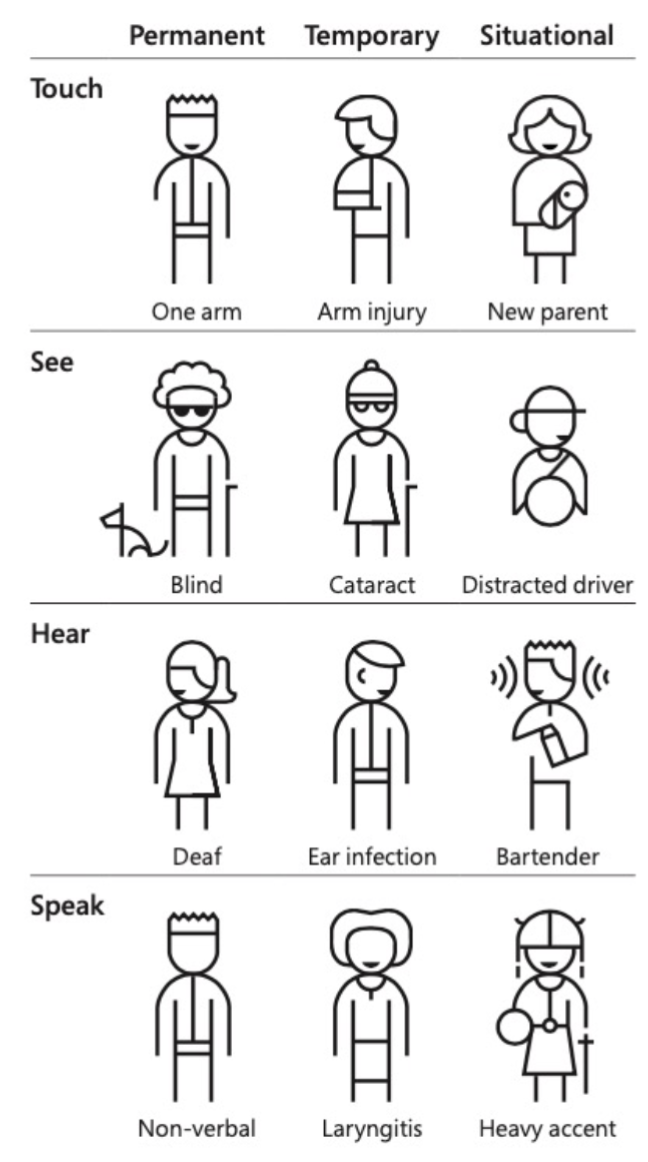
\includegraphics[scale=0.8]{lectures/wk13/img/disability_types.png}
\end{center}
Note that there are different types of Disabilities which have different extents. 

\begin{shaded}
Making sure audio can be heard for people who just are hard of hearing due to an ear infection and not only accommodating for people who are completely deaf is a necessity for accessible design.
\end{shaded}

\subsection{Solve for One, Extend to Many}
Curb Cuts (when the elevation in sidewalks goes down to meet the road) are helpful for people in wheelchairs, but are also helpful for new parents who have a baby in a stroller.

\subsubsection{Closed Captioning Usages:}
\begin{itemize}
    \item Started for deaf people
    \item Good for listening to accents
    \item Allows you to watch videos in public spaces where it's too loud to listen to audio
    \item Helpful for new language learners who do not know word pronunciations but know of the word in its spelling
\end{itemize}

\subsection{Specialized Hardware}
This can help with accessibility: Braille Display is an example of this (bumps on surfaces for blind people to feel what the display is saying).

\subsection{Visual: Screen Readers}
How do we make sure to not include the footer when reading a webpage out loud?\\
How do we `read' out loud images?
\begin{shaded}
    We can set the \texttt{alt} attribute of \texttt{<img>} tags to set what the image reads out loud. Note that this extends to give an alt text in case the image cannot load.
\end{shaded}

About 8 percent of men (one in 12) and 0.5 per cent of women (one in 200) have some form of red-green colour deficiency.

\subsubsection{Do not cause Seizures!}
Do not flash anything more than three times in a row.

\subsection{Navigable}
You can set the \texttt{tabindex} of \texttt{<div>} elements to set the sequential ordering that you navigate in when pressing the \texttt{Tab} key on your keyboard. 

    \section{Thursday, April 20th}
\subsection{Future Interfaces: Virtual and Augmented Reality}
VR has been around since the 1950s with Heilig's Sensorama.

\subsubsection{Changes to costs of VR Hardware}
However VR Arcade Games in the 1990s costed tens of thousands of dollars -- but improved technology are much cheaper now (in the hundreds of dollars or less).

\begin{important}
If the costs are not low enough, some usages of technology will not be discovered. This is yet another reason why making sure hardware is accessible is important.
\end{important}
The most obvious example of the above statement is if you want to be able to draw with brushstrokes in 3D. Would you pay \$20,000 for that? Now what if it is $\approx\$0$, then would you consider using it?

\subsection{Augmented Reality}
Definition:
\begin{shaded}
\textbf{AR} is a computer technology that augments a physical, real-world environment directly or through its indirect view with computer-generated information, including graphics, video, and sound.

AR may alter a user’s view of reality, and may also enhance one’s perception of reality.
\end{shaded}

Note that just like VR, there was a wave of AR in the '90s. The thought was that it'd see usage in car repairs/maintenance among other applications.

Microsoft Hololens2 (2019) showcases this amongst other applications (primarily in games).

\subsubsection{Video see-through AR}
Pokemon Go is the most well-known example of this. \textit{But} it did not really try to understand the scene -- it just placed a Pokemon somewhere even if it's not a realistic horizontal surface or sensible with the current lighting.

\subsubsection{HMD-based AR}
Head Mounted Display is when you have a virtual display mounted on your head. Sometimes this is paired with actual hardware, which the headset then draws on top off (in real-time), to make a more immersive experience.

\subsubsection{Hardware Complexities}
There are lots of sensors and hardware parts, especially in HMDs.

\subsection{Enabling Technologies/
Open Research}
\begin{itemize}
    \item Near-Eye Displays and Optics
    \item 3D Localization
    \item 3D Content Capturing
    \item New Human-Computer Interfaces
\end{itemize}
\begin{center}
    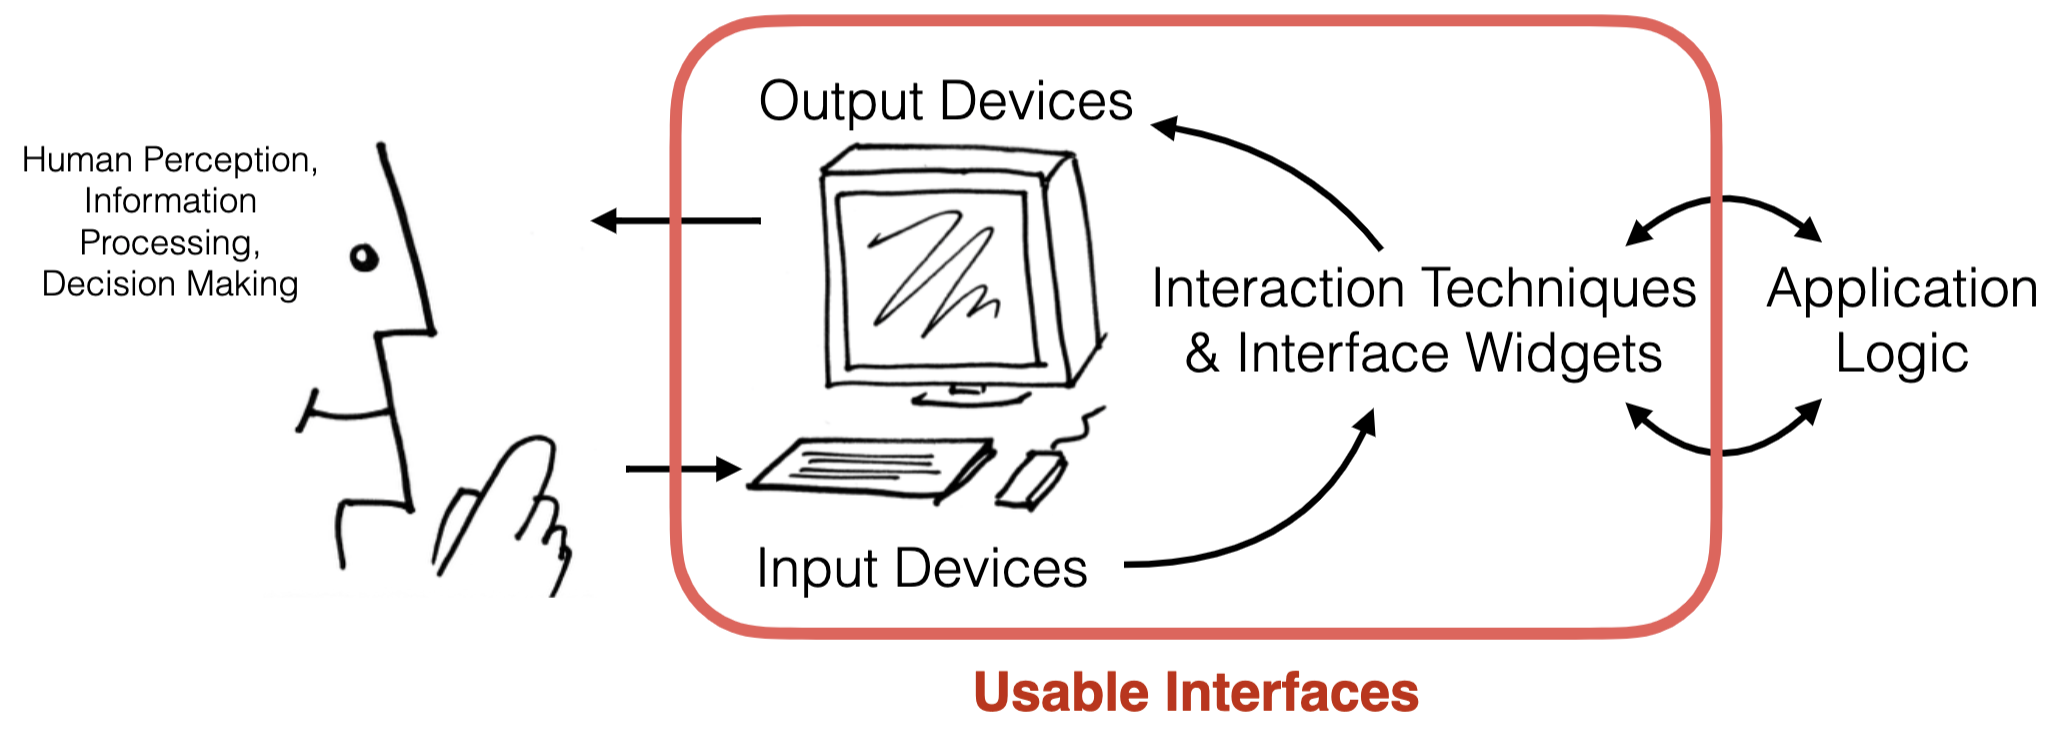
\includegraphics[scale=0.4]{lectures/wk13/img/info_proc_circled.png}
\end{center}

\subsection{Getting Input}
There are 3 important inputs to a VR/AR application: \textbf{Head, Hands and Limbs}.

\subsubsection{3D Glasses}
Red-Blue 3D glasses use light subtraction to make images seem as they come out to you -- but in the process you lose many red and blue colors and get a grayscaling effect.\\
This is known as an Anaglyph (spectral) approach.

However there is also the ``Polarization multiplexing'' approach which is much like polarizing (anti-glare) sunglasses, but with a polarizing filter on each projector.

\subsubsection{Active Shutter}
These were also glasses you could wear to see 3D video from your TV -- these were popular 10-14 years ago.

\subsection{Head-Worn Displays}
These should allow seeing-through so that you can be aware of your environment.

\subsection{Audio Displays}
\subsubsection{Auditory Cues}
\begin{itemize}
    \item Localization: psychoacoustic process of determining direction and location from
which sound emanates
\item Binaural cues:
  \begin{itemize}
    \item ITD interaural time difference
    \item IIT - interaural intensity difference
    \item HRTF - head related transfer function (physical shape of ears, ear canals)
    \item Reverberation
    \item Intensity
  \end{itemize}
\end{itemize}

\[
I \propto \frac{1}{r^2}
\]
where $I$ is the sound pressure level, and $r$ is distance.

HRTF measurement: For far objects, radius less
important. Function of sound frequency and
position: azimuth, elevation,
radius.

\subsection{Reverberation}
Early reflection: localization\\
Long tail late reflection: room characterization

\subsection{Haptic Displays}
\begin{itemize}
    \item Simulate the the physical interaction between the user and objects
    \item Encompasses sensations of force, touch, vibration, temperature
\end{itemize}
Core challenge: cues for particular categories are very different from other categories.

\subsection{Gustation and Olfaction
Displays}
\begin{shaded}
Can we simulate smell and taste?
\end{shaded}
Current answer: No.

Sound: Air pressure variations over time (which is 1-dimensional).
Vision: Red-Green-Blue pixels (which are 3-dimensional).

But smells are a much more complicated dimensionality and carrying a backpack with thousands of smells in jars is not really feasible.

With taste, we have a subset spanned by descriptions (such as salty, sour, sweet, etc) but this does not generate a basis.

\subsection{Professor Hartmann's PhD students' work: Pointing \& Selection in 3D}
How do we select stuff that is further away:
\begin{itemize}
    \item Shrink stuff down
    \item Cast a ray into the scene
\end{itemize}
There has been success in making arms that reach out beyond an actual human's reach -- much like Inspector Gadget's mechanical arms.

Remember that since we are doing a \textit{simulation}, we can alter the laws of physics that are written in the code.

Results: you can control multiple bodies at the same time -- with a natural feeling, despite it being an action that can never happen in reality. Cognitive Science has yet to give an answer to why that is.

\subsection{Bi-manual Scaling}
Pinch-to-zoom but with 2 controllers -- allows us to scale the world up or down.

    \section{Tuesday, April 25th: Career Panel}
\subsection{Speaker List}
We have Speakers from:
\begin{itemize}
    \item Heidi Dong (\href{https://www.linkedin.com/in/heididong/}{LinkedIn}), Software Engineer, Frontend at The New York Times

    \item Janaki Vivrekar (\href{https://janakivivrekar.com/}{Personal}, \href{https://www.linkedin.com/in/janaki-vivrekar/}{LinkedIn}), Software Engineer at Amplitude

    \item Sonia Uppal (\href{https://www.linkedin.com/in/soniau/}{LinkedIn}), Software Engineer at Meta

    \item Emily Pedersen (\href{https://www.emilypedersen.me/}{Personal}, \href{https://www.linkedin.com/in/epedersen1/}{LinkedIn}), SW Engineering Program Manager at Apple
\end{itemize}

\subsection{Midterm \#2 Graded}
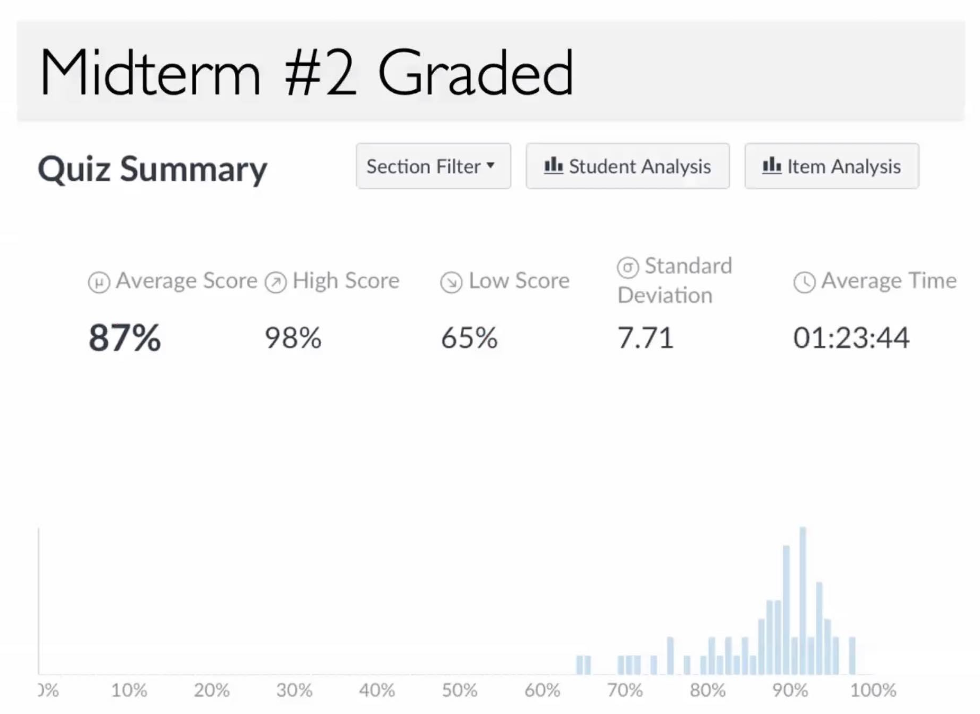
\includegraphics{lectures/wk14/img/mt2_distro.png}

\subsubsection{Regrades}
Same as midterm 1.

\subsubsection{Course Standing}
If you have any concerns about your standing in the
course and your ability to graduate, please get in
touch with us proactively via private message on Ed
Discussion.

\subsection{End of the Semester}
Course summary and next steps on April 27\\
Section: Submit update including demo video this week \textbf{before section}!

\subsection{Design Showcase}
Design Showcase runs Wed-Fri of RRR week every semester. The Jacobs Institute will promote all courses and projects to the public.

Our presentation slot:\\
Design Showcase Session C:\\
Wednesday, 5/3 - 2-3:30pm / Jacobs Hall Room 310

Poster: Due Monday 5/1 11:59am (noon) if you want us to print it!

\subsection{Poster Details}
See \href{https://bcourses.berkeley.edu/courses/1523321/assignments/8584015}{bcourses}.

\subsection{Final Demo Details}
See \href{https://bcourses.berkeley.edu/courses/1523321/assignments/8578979}{bcourses}.

\subsection{Q\&A}
How has ChatGPT changed the way you worked?
\begin{shaded}
Most companies do not allow you to use ChatGPT for obvious reasons but on the side it has been cool to play around with.
\end{shaded}

What courses were most useful?
\begin{shaded}
I work in TypeScript which was not taught in any class at Cal but look into taking DeCals and others, see:
\begin{itemize}
    \item 
\href{https://www.figma.com/proto/LIWnxQaKzQkYD5k5wpP8oA/classes-i've-taken}{https://www.figma.com/proto/LIWnxQaKzQkYD5k5wpP8oA/classes-i've-taken}

    \item 
\href{https://vivrekar.medium.com/discovering-human-computer-interaction-at-uc-berkeley-9fc211145638}{https://vivrekar.medium.com/discovering-human-computer-interaction-at-uc-berkeley-9fc211145638}
\end{itemize}
\end{shaded}

    \section{Thursday, April 27th}
\subsection{Last Class... but wait there's more}
CS 160 has their Jacobs Spring Design Showcase at Studio 310 on Session C (2-3:30 PM).

Note that this is the same classroom where regular lecture is held but the date is different: Wednesday May 4th.

\subsection{Final Deliverables}
What should you submit on \textbf{May 10th}?
\begin{itemize}
    \item \textbf{Writeup:} Now that you have a working app, get feedback from \textbf{3} users, write up what you learned and would change.
    \item \textbf{Video:} Record a demo video of the final application.
    \item \textbf{Source Code:} Remind us of the link to your repo, make sure you have a \texttt{README.txt}.
\end{itemize}

\subsection{Takeaways}
\subsubsection{Why UI is Important}
Major part of work for ``real'' programs
\begin{itemize}
    \item Approximately 50\%
\end{itemize}
You will work on “real” software
\begin{itemize}
    \item Intended for people other than yourself
\end{itemize}
Bad user interfaces cost
\begin{itemize}
    \item Money (5\%$\uparrow$ satisfaction $\implies$ up to 85\%$\uparrow$ profits)
    \item Lives
\end{itemize}
User interfaces hard to get right
\begin{itemize}
    \item People are unpredictable
\end{itemize}

\hrulefill

So what should you do then?\\
Answer: \textbf{Iterative Design}

Finally, don't use intuition for design -- instead observe the user in context. \\
Also separate the designer's conceptual model from the users' (which is from experience \& usage).

\subsection{Future Coursework for Undergraduates}
BCDI: Berkeley Certificate in Design Innovation
\begin{itemize}
    \item Interdisciplinary certificate (like minor)
    \item 4 courses, CS160 counts as one of them -- you are 25\% done!
    \item Look at DES INV courses (they all count)
    \item \href{https://bcdi.berkeley.edu}{https://bcdi.berkeley.edu}
\end{itemize}

Decals and student Orgs:
\begin{itemize}
    \item Web Design Decal \href{https://wdd.io}{https://wdd.io}
    \item InnoD Decals \href{https://www.innovativedesign.club}{https://www.innovativedesign.club}
    \item Berkeley Innovation: \href{https://www.berkeleyinnovation.org}{https://www.berkeleyinnovation.org}
    \item Extended Reality @ Berkeley: \href{https://xr.berkeley.edu}{https://xr.berkeley.edu}
\end{itemize}

\subsubsection{Graduate School}
Thinking about graduate school? Check out
\begin{itemize}
    \item Berkeley MDes – Master in Design
    \item Berkeley MEng – Visual Computing
    \item Berkeley MIMS
    \item Berkeley PhD in CS; iSchool
\end{itemize}

Other Universities with top HCI programs: CMU, U Dub, Stanford, GTech, MIT,
UMD, etc.

\subsubsection{What if I am a Graduate student?}
Relevant Graduate Courses at Berkeley
\begin{itemize}
    \item CS294-137 Immersive Computing (Yang, Hartmann)\footnote{only ugrads allowed will be those who have taken CS 160 -- and by petition}
    \item CS294-184 Building User-Centered Programming Tools (Chasins)\footnote{only for PhDs}
    \item NWMEDIA 203 Critical Making (Paulos)
    \item CS260B Topics in HCI Research (Paulos, Hartmann)
    \item INFO 214: User Experience Research (Fadden)
    \item INFO 247: Information visualization and presentation (Hearst)
    \item INFO C262: Tangible User Interfaces (Ryokai)
    \item INFO C265: Interface Aesthetics (Ryokai)
    \item INFO 290: Human-Centered AI (Salehi)
    \item and many more!
\end{itemize}
\begin{important}
INFO 213 is similar to CS160 – only take one
\end{important}

\subsection{Q\&A:}
\begin{shaded}
Q: What is the best way to get into SWE as an M.Eng.

A: Take CS 169
\end{shaded}

\subsection{Course Evaluations}
Please fill out \href{https://course-evaluations.berkeley.edu/}{https://course-evaluations.berkeley.edu/}

\end{document}
